% RVD: design notes for a Voronoi and restricted Voronoi engine you can look inside.
%
% Build with pdflatex, twice (the second pass resolves the cross-references):
%
%   latexmk -pdf DESIGN.tex        or        pdflatex DESIGN.tex && pdflatex DESIGN.tex
%
% No BibTeX run is needed: the references are a thebibliography list, which natbib reads
% in author-year form.
\documentclass[11pt,a4paper]{article}

\usepackage[T1]{fontenc}
\usepackage[utf8]{inputenc}
\usepackage{lmodern}
\usepackage[british]{babel}
\usepackage[a4paper,margin=2.4cm]{geometry}
\usepackage{microtype}
\usepackage{amsmath,amssymb,mathtools}
\usepackage{array,booktabs,tabularx,xltabular}
\usepackage[shortlabels]{enumitem}
\usepackage{xcolor}
\usepackage{tikz}
\usetikzlibrary{arrows.meta,positioning,calc}
\usepackage{caption}
\usepackage[round,authoryear]{natbib}
\usepackage{url}
\usepackage[colorlinks,linkcolor=blue!50!black,citecolor=blue!50!black,urlcolor=blue!50!black]{hyperref}

% --- notation -------------------------------------------------------------------------
\newcommand{\code}[1]{\texttt{#1}}          % identifiers; escape _ as \_
\newcommand{\R}{\mathbb{R}}
\newcommand{\norm}[1]{\lVert #1\rVert}
\newcommand{\secref}[1]{\S\ref{#1}}
\newcommand{\Secref}[1]{\S\ref{#1}}          % the same, at the start of a sentence

% --- tables ----------------------------------------------------------------------------
% L: a ragged-right X column, for text that wraps.
\newcolumntype{L}{>{\raggedright\arraybackslash}X}
\newcolumntype{P}[1]{>{\raggedright\arraybackslash}p{#1}}
\renewcommand{\arraystretch}{1.15}
\setlength{\LTpre}{6pt}
\setlength{\LTpost}{6pt}

% --- lists and boxes -------------------------------------------------------------------
\setlist{itemsep=2pt,topsep=4pt}
\newcommand{\keybox}[1]{%
  \begin{center}\fbox{\begin{minipage}{0.94\linewidth}\centering\smallskip #1\smallskip\end{minipage}}\end{center}}

\title{\textbf{RVD}\\[0.4em]
  \large Design notes for a Voronoi and restricted Voronoi engine you can look inside}
\author{}
\date{30 September 2026}

\begin{document}
\maketitle

\keybox{\raggedright\small
  \textbf{Status.} Design only, no code yet. Written against \code{mesh-viewer} at
  \code{18b9619} and \code{mesh-dev} at \code{dc7151c}. Everything said about the viewer was
  checked against its source, and everything said about the mathematics has a reference at the
  end.}

This document is meant to be read from start to finish once, then used for reference.
\Secref{sec:idea} is the whole idea on one page. \Secref{sec:math} is the mathematics, kept to
what the design needs. Sections~\ref{sec:arch} to~\ref{sec:algorithms} are the system: its
layers, its data, its predicates, its algorithms. \Secref{sec:viewer} is how it sits on your
viewer. \Secref{sec:plan} is the order to build it in, and \secref{sec:testing} is how each
step is tested. \Secref{sec:generalisation} answers the question you asked directly: how the
plain Voronoi diagram becomes a restricted one, and why the design is built so that this step
is small.

\tableofcontents
\clearpage

% ======================================================================================
\section{The idea on one page}\label{sec:idea}

You are building a C++17 library, and a mesh-viewer host program around it. The library
computes the Voronoi diagram of a set of points, the \emph{seeds}, optionally with a weight each
(a \emph{power} or \emph{Laguerre} diagram). It computes it clipped to a box, restricted to a
triangle surface, or restricted to the inside of a tetrahedral mesh. From the cells it produces
a mesh to look at, the mass and centroid of every cell, the restricted Delaunay triangulation,
and a list of everything that is wrong with the result. On top of that sit the optimisers that
make Voronoi diagrams useful: Lloyd and L-BFGS for centroidal Voronoi tessellations, and Newton
on the weights for semi-discrete optimal transport.

One sentence organises the whole design:

\keybox{\textbf{A Voronoi cell is a convex polytope cut out by half-spaces.\\
  A restricted cell is those same half-spaces applied to the pieces of a domain.}}

So the engine is one \emph{clipper}, fed by a \emph{neighbour oracle} that says which
half-spaces bound each cell, and feeding a set of \emph{consumers} that turn clipped pieces into
whatever you want (figure~\ref{fig:pipeline}).

\begin{figure}[ht]
\centering
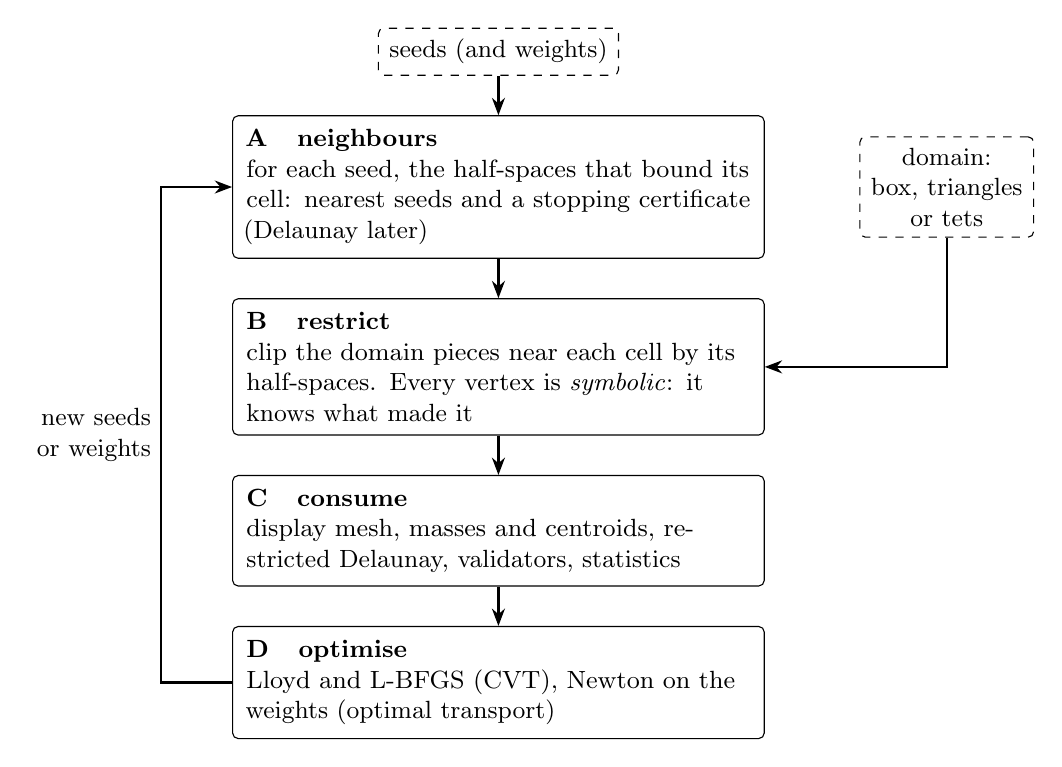
\begin{tikzpicture}[
    node distance=5mm and 8mm,
    stage/.style={draw, rounded corners=2pt, align=left, inner sep=5pt, text width=6.4cm,
                  font=\small},
    input/.style={draw, dashed, rounded corners=2pt, align=center, inner sep=4pt,
                  font=\small},
    arr/.style={-{Stealth[length=2.2mm]}, thick}]
  \node[input] (seeds) {seeds (and weights)};
  \node[stage, below=of seeds] (A) {\textbf{A\quad neighbours}\\
    for each seed, the half-spaces that bound its cell: nearest seeds and a stopping
    certificate (Delaunay later)};
  \node[stage, below=of A] (B) {\textbf{B\quad restrict}\\
    clip the domain pieces near each cell by its half-spaces. Every vertex is
    \emph{symbolic}: it knows what made it};
  \node[stage, below=of B] (C) {\textbf{C\quad consume}\\
    display mesh, masses and centroids, restricted Delaunay, validators, statistics};
  \node[stage, below=of C] (D) {\textbf{D\quad optimise}\\
    Lloyd and L-BFGS (CVT), Newton on the weights (optimal transport)};
  \node[input, right=12mm of A] (domain) {domain:\\box, triangles\\or tets};
  \draw[arr] (seeds) -- (A);
  \draw[arr] (A) -- (B);
  \draw[arr] (domain) |- (B.east);
  \draw[arr] (B) -- (C);
  \draw[arr] (C) -- (D);
  \draw[arr] (D.west) -- ++(-9mm,0) |- node[pos=0.25, left, align=right, font=\small]
    {new seeds\\or weights} (A.west);
\end{tikzpicture}
\caption{The four stages. A computes the Voronoi diagram in the domain's bounding box, B
restricts it to the domain, C turns the clipped pieces into results, and D moves the seeds or
the weights and starts again.}
\label{fig:pipeline}
\end{figure}

Three decisions shape everything after this page.

\begin{enumerate}
\item \textbf{A Voronoi diagram in a box is a restricted Voronoi diagram}, whose domain happens
  to be one convex piece. So the Voronoi maker you build first is not a separate program that
  the RVD later replaces. It is stage A and stage B running on the simplest possible domain, and
  every line of it survives into the RVD.
\item \textbf{Every vertex is symbolic.} A vertex is stored as \emph{what defines it}
  (``triangle 812, where the bisectors of seeds 4--17 and 4--23 cross it''), with its
  coordinates only as a derived, display-grade copy. Every decision the algorithm takes is a
  predicate evaluated exactly, from the input numbers alone. That single choice buys exactness,
  vertex welding without tolerances, the dual complex for free, and a debugger that can say why
  any vertex exists.
\item \textbf{The viewer is a host concern.} The core never includes a GL header, exactly as in
  mesh-dev. A result is an immutable \emph{generation} that the host publishes through
  \code{MeshSource} and \code{OverlaySource}. The viewer does not change for phase one. Two
  small, general viewer extensions are proposed for later, in \secref{ssec:extensions}, and
  neither is required.
\end{enumerate}

What will make it more than another Voronoi code (\secref{sec:interesting}): a
\emph{robustness microscope} that shows which predicates needed exact arithmetic and where the
input was degenerate. A \emph{closed-ball inspector} that shows exactly where your sampling is
too coarse for the restricted Delaunay triangulation to be a valid mesh. \emph{Cell replay}, to
watch one cell being clipped bisector by bisector. Optimisation you can watch converge live. And
results that are bit-identical on one thread and on sixty-four, tested against constants known
in closed form.

% ======================================================================================
\section{What exists, and the gap}\label{sec:exists}

Your impression that there is no good RVD software online is fair, with one large exception.

{\small
\begin{xltabular}{\linewidth}{@{}P{2.3cm} L L@{}}
\toprule
software & what it does well & why it is not what you want \\
\midrule
\endhead
\textbf{Geogram} (B.~Lévy, Inria)
  & The reference. Delaunay in 3D, restricted Voronoi diagrams on surfaces and volumes, power
    diagrams, exact predicates through its Predicate Construction Kit, CVT remeshing
    (\code{vorpalite}), and semi-discrete optimal transport
  & Dense code inside a large framework with its own mesh type, attribute system and
    conventions. Built to be fast and correct, not to be read, changed or looked inside:
    nothing in it shows you, on the mesh, why a given vertex exists or where exact arithmetic
    was needed. You already benchmark against it (\code{mesh-dev/\allowbreak tests/\allowbreak bench\_vs\_geogram.cpp}),
    and it should stay your second opinion here too (\secref{ssec:geogram}) \\
\textbf{CGAL}
  & Delaunay and regular triangulations in 3D with exact predicates, and mesh generation that
    uses restricted Delaunay triangulations internally
  & As far as I know it has no public restricted Voronoi diagram of a triangle mesh for
    arbitrary seeds: no cells restricted to a surface, no cell integrals, no CVT on a
    surface \\
\textbf{voro++} \citep{rycroft2009}
  & Fast, well-documented 3D Voronoi cells, one at a time, in boxes and simple walls
  & Floating-point tolerances, and no triangle-mesh or tet-mesh domains. It does radical
    (power) diagrams, but has no CVT or transport on top \\
\textbf{Qhull}, \code{scipy.\allowbreak spatial.\allowbreak Voronoi}
  & Convex hulls, Delaunay triangulations, unbounded Voronoi diagrams
  & No clipping and no restriction. Unbounded cells come back with a vertex ``at infinity'' \\
GPU research codes \citep{ray2018,basselin2021}
  & Very fast Voronoi and restricted power diagrams, ``meshless'', one cell per thread
  & Floating point, and written for their papers' experiments rather than as libraries. Their
    \emph{algorithm}, though, is the one this design adopts for stage A
    (\secref{sssec:meshless}) \\
\bottomrule
\end{xltabular}}
Geogram is at \url{https://github.com/BrunoLevy/geogram}, and CGAL at \url{https://www.cgal.org}.

The gap is not speed. It is an RVD engine you can \textbf{read, trust, test, and look inside},
with the knobs reachable, in the style of your own code. mesh-dev's rule applies: the header
says why, the \code{.cpp} says how, and nothing hides an idea behind an abstraction.

% ======================================================================================
\section{The mathematics the design rests on}\label{sec:math}

Kept to what the design needs. Everything here is standard, and the references at the end have
the proofs.

\subsection{Cells are intersections of half-spaces}\label{ssec:halfspaces}

Take seeds $p_1,\dots,p_n$ in $\R^3$, each with a weight $w_i$ (zero for an ordinary Voronoi
diagram). The \emph{power distance} from a point $x$ to seed $i$ is
\[
  \pi_i(x) = \norm{x - p_i}^2 - w_i ,
\]
and the cell of seed $i$ is every point at least as close to $i$ as to any other seed:
\[
  V_i = \{\, x : \pi_i(x) \le \pi_j(x) \text{ for every } j \,\}.
\]
Expand one of those conditions and the $\norm{x}^2$ on both sides cancels:
\[
  \pi_i(x) \le \pi_j(x) \iff 2\,x\cdot(p_j - p_i) \le \norm{p_j}^2 - \norm{p_i}^2 + w_i - w_j .
\]
That is a \textbf{half-space}, bounded by the \emph{bisector} plane of $i$ and $j$. So every
cell is an intersection of half-spaces, which makes it a convex polytope: possibly unbounded (a
seed on the convex hull of the seeds), and, with weights, possibly empty, or not containing its
own seed.

Only a few of the $n-1$ half-spaces matter: the ones whose plane actually supports a face of
the cell. Those seeds are the cell's \emph{neighbours}. For uniformly random seeds in 3D a cell
has on average $48\pi^2/35 + 2 \approx 15.54$ faces and $96\pi^2/35 \approx 27.07$ vertices
\citep{meijering1953}. That number is why the whole problem is cheap. A cell is decided by
about fifteen planes out of millions, and finding those fifteen is stage A.

One more fact stage A needs. The bisector of $i$ and $j$ lies at signed distance
\[
  t_{ij} = \frac{d_{ij}^2 + w_i - w_j}{2\,d_{ij}}, \qquad d_{ij} = \norm{p_j - p_i},
\]
from $p_i$, which is $d_{ij}/2$ without weights (with weights it is negative when $p_i$ itself is
on $j$'s side). A plane farther from $p_i$ than every point of the cell cannot cut it. That is
the \emph{security radius} test of \secref{sssec:meshless}.

\subsection{Restriction is clipping, piece by piece}\label{ssec:restriction}

The domain $\Omega$ is where you want the diagram: a box $B$, a triangulated surface $S$, or the
inside of a tetrahedral mesh. The restricted cell is $V_i \cap \Omega$. Write the domain as a
union of convex \emph{pieces} $P_t$: the box itself, or the triangles of $S$, or the tets. Then
\[
  V_i \cap \Omega = \bigcup_t \, (V_i \cap P_t).
\]
Each $V_i \cap P_t$ is convex, because both factors are. It is exactly \emph{the piece $P_t$
clipped by the half-spaces of cell $i$}, the same half-spaces as in \secref{ssec:halfspaces}.
This is the step from Voronoi to RVD, and it is only this. A restricted cell is a union of convex
clipped pieces. On a curved or non-convex domain that union can be non-convex, and even
\textbf{disconnected} (a thin plate: one cell reaches both faces). The traversal in
\secref{ssec:stageB} is built not to assume otherwise.

Vocabulary: a \emph{restricted Voronoi diagram} (RVD) usually means restricted to a surface.
Its volume counterpart is also called the \emph{clipped Voronoi diagram} \citep{yan2013}. Here
both are one thing with two kinds of piece.

\subsection{The dual: the restricted Delaunay triangulation}\label{ssec:rdt}

The \emph{restricted Delaunay triangulation} (RDT) records which cells meet on the domain. On a
surface, the triangle $\{i,j,k\}$ is in the RDT when $V_i \cap V_j \cap V_k \cap S$ is non-empty.
Generically that is a point where the Voronoi edge of $i$, $j$ and $k$ (part of the line of
points equidistant from all three) pierces the surface. In a volume, the tet $\{i,j,k,l\}$ is in
it when the Voronoi vertex of those four seeds lies inside $\Omega$. The RDT of a good CVT on a
surface is the classic isotropic remesh \citep{yan2009}. The RDT of a clipped Voronoi diagram
is, when the sampling is fine enough, a Delaunay tet mesh of $\Omega$.

When is the RDT a valid mesh of $S$, with no holes, folds or extra handles? The \emph{closed ball
property} \citep{edelsbrunner1997} answers it. If every restricted cell $V_i \cap S$ is a disk,
every pair of cells shares at most one arc, and every triple meets in at most one point, then the
RDT is homeomorphic to $S$. Dense enough sampling guarantees it: an $\varepsilon$-sample does,
for small enough $\varepsilon$ \citep{amenta1999}. Coarse sampling violates it locally, and that is exactly where remeshing goes
wrong. \Secref{ssec:closedball} turns this property into a tool.

\subsection{What is integrated, and why}\label{ssec:integrals}

With a density $\rho$ on $\Omega$ (one if you don't care), every restricted cell has
\begin{align*}
  m_i &= \int_{V_i\cap\Omega} \rho(x)\,dx                         && \text{its mass,}\\
  c_i &= \frac{1}{m_i}\int_{V_i\cap\Omega} \rho(x)\,x\,dx         && \text{its centroid,}\\
  E_i &= \int_{V_i\cap\Omega} \rho(x)\,\norm{x - p_i}^2\,dx       && \text{its energy,}
\end{align*}
and every pair of neighbours has a \emph{facet measure}: the $\rho$-weighted area of
$V_i \cap V_j \cap \Omega$, or its length on a surface.

The total energy $E = \sum_i E_i$ is the \emph{centroidal Voronoi tessellation} (CVT) energy.
Its gradient is $\partial E/\partial p_i = 2\,m_i\,(p_i - c_i)$ \citep{du1999}, so a CVT, a
diagram whose seeds sit at their centroids, is a critical point. \textbf{Lloyd's algorithm} is
the fixed-point iteration $p_i \leftarrow c_i$. It never raises the energy, but it converges
slowly. \textbf{L-BFGS} on $E$ with that gradient is far faster, because $E$ is $C^2$ on convex
domains with a smooth density, and in most situations met in practice \citep{liu2009}.

On a surface, $c_i$ lies off the surface. The \emph{constrained} CVT \citep{du2003} keeps each
seed on the surface by moving it to the point $z$ of the surface nearest to $c_i$. That point is
exactly the best position on the surface for that cell, because for any $z$
\[
  \int_{V_i\cap S} \rho(x)\,\norm{x - z}^2\,dx
  = \int_{V_i\cap S} \rho(x)\,\norm{x - c_i}^2\,dx + m_i\,\norm{c_i - z}^2 ,
\]
so Lloyd stays monotone, provided the nearest point is the true, global one (mesh-dev's BVH
query returns that). Whether seeds should stay on the surface belongs to the application, and a
remesh wants them there. So it is a parameter, not a hidden default.

With a density, CVT cells shrink where $\rho$ is large, with a size proportional to
$\rho^{-1/(d+2)}$ in dimension $d$ \citep{du1999}. That is how an adaptive remesh or sampling is
steered.

\subsection{Optimal transport: why the weights exist from day one}\label{ssec:ot}

Give each seed a target mass $\nu_i$, the $\nu_i$ summing to the mass of $\Omega$.
\emph{Semi-discrete optimal transport} looks for the weights $w$ for which every power cell has
exactly its target mass: $m_i(w) = \nu_i$. The mass map $w \mapsto m(w)$ is, up to sign, the
gradient of a concave function, the Kantorovich dual, so solving $m(w) = \nu$ is maximising that
function. Its Hessian is, again up to sign, a \textbf{graph Laplacian on the neighbour graph},
whose edge weights are
\[
  \frac{\text{the $\rho$-weighted area of the facet between $i$ and $j$}}{2\,d_{ij}}
\]
for the cost $\norm{x-y}^2$. So one RVD pass gives the function, the gradient and the Hessian
together. A damped Newton method converges globally, under mild conditions on the density
\citep{kitagawa2019}, and \citet{levy2015} gives the algorithm in 3D.

Equal-volume cells are what Lagrangian fluid schemes built on power diagrams need: \emph{power
particles} \citep{degoes2015}, and Lévy's constant-volume free-surface meshes
\citep{levy2022}. Blue-noise sampling is optimal transport too \citep{degoes2012}. That is the
reason every data structure below carries a weight per seed even while every weight is zero.
Adding them later would mean touching every predicate.

\subsection{Degeneracy, stated honestly}\label{ssec:degeneracy}

Everything above assumes \emph{general position}: no five seeds on one sphere, no domain vertex
on a bisector, no surface triangle lying inside a bisector plane. Real inputs break it all the
time. Lattices, symmetric seeds, seeds placed on mesh vertices, and a flat face of a CAD surface
lying in a bisector plane are all exactly degenerate. A cubic lattice is degenerate at
\emph{every} Voronoi vertex, where eight seeds are equidistant.

The design answers this once, in \secref{ssec:sos}, with symbolic perturbation. Exact ties are
broken as if the input had been moved by an infinitesimal amount, consistently for every
predicate. The result is the diagram of that perturbed input. The measures are unchanged, and
the combinatorics are generic, sometimes with zero-length edges and zero-area faces where the
true diagram has a vertex of high degree. The whole point of \secref{sec:predicates} is that the
algorithms of \secref{sec:algorithms} \textbf{may assume general position, and the input never
has to provide it.}

% ======================================================================================
\section{Architecture}\label{sec:arch}

\subsection{Layers, and which way they depend}\label{ssec:layers}

{\small
\begin{xltabular}{\linewidth}{@{}P{3.2cm} L@{}}
\toprule
directory & contents \\
\midrule
\endhead
\code{ext/mesh-viewer} & the viewer, a submodule, pulled in exactly as mesh-dev does it \\
\code{src/kernel/}     & numbers and predicates: filtered doubles, exact fallback, symbolic
                         perturbation, counters. Depends on nothing \\
\code{src/points/}     & seeds and weights, the spatial index (nearest seeds), Morton order,
                         samplers (uniform, lattice, on a surface, from a file) \\
\code{src/domain/}     & \code{Box}, \code{SurfaceDomain}, \code{VolumeDomain}: convex pieces,
                         their features (vertices, edges, faces), adjacency, an AABB tree \\
\code{src/cells/}      & the two clippers, \code{ConvexCell} (3D) and \code{ClippedPolygon} (on
                         a triangle), and symbolic vertices \\
\code{src/diagram/}    & stage A (neighbour oracles) and stage B (traversals) \\
\code{src/consumers/}  & display mesh, integrator, restricted Delaunay, validators,
                         statistics \\
\code{src/optimize/}   & Lloyd, L-BFGS on the CVT energy, Newton on the weights \\
\code{src/io/}         & readers (mesh-dev's) and writers (\code{.obj}, \code{.msh},
                         \code{.csv}) \\
\code{src/app/}        & the mesh-viewer host: sources, panels, picking, generations \\
\code{tests/}          & one source file per suite, with mesh-dev's \code{check()} harness \\
\code{docs/}           & this document, and what grows from it \\
\bottomrule
\end{xltabular}}

Each directory under \code{src/} depends only on the ones listed above it, and only
\code{app/} sees the viewer. Nothing outside \code{app/} includes a GL or ImGui header. The build
has the same shape as mesh-dev's: a static library \code{rvd\_core} (everything but
\code{app/}), the executable \code{rvd}, and test binaries that link only the core. A machine
with no display can build and test all of the mathematics.

\subsection{What to reuse from mesh-dev}\label{ssec:reuse}

A lot of what this needs already exists in mesh-dev, written in the style you want here.

{\small
\begin{xltabular}{\linewidth}{@{}P{5.2cm} L@{}}
\toprule
mesh-dev piece & what RVD uses it for \\
\midrule
\endhead
\code{mesh/surface\_mesh.h}, \code{mesh/tet\_mesh.h}
  & the domains' pieces and adjacency: fixed connectivity, \code{neighbor(t, e)} and
    \code{neighbor(t, f)}, \code{kEdges} and \code{kFaces}, positively oriented tets, a
    revision \\
\code{mesh/vertex\_incidence.h}
  & the CSR pattern, for the neighbour graph and the grid's bins \\
\code{io/} (\code{MeshData}, the \code{.msh} and \code{.obj} readers)
  & loading domains, and seeds from a file \\
\code{mesh/morton\_order.h}
  & spatial order for seeds and domain pieces: locality for stages A and B \\
\code{core/hash.h}
  & \code{mix64} and \code{pow2\_at\_least}, for the open-addressing table that welds symbolic
    vertices \\
\code{core/parallel.h}
  & \code{deterministic\_sum}, for every global sum \\
\code{geometry/surface\_bvh.h}, \code{geometry/winding\_number.h}
  & ``is this seed inside, and how far from the boundary'': the shortcut that lets interior
    cells skip restriction entirely (\secref{ssec:stageB}). The winding numbers follow
    \citet{barill2018} \\
\code{tests/test\_support.h}
  & \code{check}, \code{report\_checks}, \code{tet\_cube}, \code{sphere} \\
\code{ext/lbfgs-lite}
  & L-BFGS for the CVT \\
\bottomrule
\end{xltabular}}

How to take them: at first, point CMake at the mesh-dev sources by path, with an option such as
\code{RVD\_MESH\_DEV\_DIR}, the way \code{MESH\_DEV\_VIEWER\_DIR} points mesh-dev at another
viewer checkout. Compile only the dozen files needed. Do not copy them, because copies drift. If
both projects keep needing them, split a small \code{mesh-core} repository out, the way you
split the viewer out on 29 September.

\subsection{The stages and what each one produces}\label{ssec:stages}

{\small
\begin{xltabular}{\linewidth}{@{}P{2.2cm} L L P{2.1cm}@{}}
\toprule
stage & reads & produces & cost \\
\midrule
\endhead
\textbf{seeds}
  & a sampler's parameters, or a file
  & \code{PointSet}: positions, weights, a revision
  & $O(n)$ \\
\textbf{A. neighbours}
  & \code{PointSet}, and the bounding box $B$ of the domain
  & \code{NeighbourGraph}: for every seed, the seeds whose bisectors bound its cell inside $B$
  & $O(nk)$ for $k$ neighbours tried \\
\textbf{B. restrict}
  & \code{NeighbourGraph}, \code{Domain}
  & a \emph{stream} of clipped pieces: (seed, piece, symbolic polygon or polyhedron)
  & $O(\text{output})$ \\
\textbf{C. consume}
  & that stream
  & whatever the attached consumers build: display mesh, integrals, facet measures, RDT,
    validation report, predicate statistics
  & $O(\text{output})$ \\
\textbf{D. optimise}
  & integrals and facet measures
  & new positions (CVT) or new weights (transport)
  & one A + B + C per iteration \\
\bottomrule
\end{xltabular}}

On a box domain, stage B is almost nothing. Each cell from stage A \emph{is} its restricted
cell, because the box is the one convex piece. That is the first decision of \secref{sec:idea},
in table form.

\subsection{Stage B streams, and consumers listen}\label{ssec:streams}

Stage B does not build ``the RVD'' as a data structure. It hands every clipped piece, as it is
made, to the consumers attached to this run, and forgets it. Geogram's RVD works the same way,
through callbacks. This matters for three reasons:

\begin{itemize}
\item \textbf{Size.} The RVD of a million seeds on a million triangles is several million
  polygons. An optimiser needs only a mass and a centroid per seed, which is 32 bytes.
\item \textbf{Composition.} A run is ``stage B plus a list of consumers''. A Lloyd step attaches
  the integrator. A display refresh attaches the mesh builder. Validation attaches the validator
  to either. The traversal is written once.
\item \textbf{Honesty.} The display mesh is one consumer among others, so the picture cannot show
  something the integrals did not see.
\end{itemize}

\subsection{Freshness}\label{ssec:freshness}

Every derived structure records the revisions it was built from: the point set's, the domain's,
and a hash of the parameters that matter. It is refreshed through one \code{update} that
compares them and rebuilds only what is stale. This is \code{SurfaceQueries::update} in
mesh-dev, where asking is the same act as making sure. Here it covers the spatial index, the
neighbour graph and the last generation.

\subsection{Parallel, and bit-identical}\label{ssec:determinism}

mesh-dev's rule carries over unchanged: \textbf{results are identical on one thread and on
sixty-four.} The design keeps it by structure rather than by care:

\begin{itemize}
\item Stage A and the default stage B run \emph{per seed}. A seed's result depends only on the
  input, and is written into that seed's own slot. Scheduling cannot change it.
\item Every list that feeds a later loop is sorted by seed id before use (neighbour lists, for
  instance), so traversal order never depends on which thread got there first.
\item Every sum over seeds or pieces is a \code{deterministic\_sum}, or is reduced in index
  order.
\item Predicate counters are integers, so the order they are added in does not matter.
\item A test runs the same diagram on 1 and on $N$ threads and compares a hash of every output
  (\secref{ssec:determinismtest}).
\end{itemize}

% ======================================================================================
\section{Data structures}\label{sec:data}

Plain arrays indexed by plain integers, as in \code{TetMesh}, with no attribute store.
Everything is double precision, with \code{glm::dvec3} as three packed doubles (the same
\code{static\_assert} as \code{tet\_mesh.h}).

\subsection{\texorpdfstring{\code{PointSet}}{PointSet}: the seeds}\label{ssec:pointset}

{\small
\begin{xltabular}{\linewidth}{@{}P{2.2cm} L L@{}}
\toprule
field & what & why \\
\midrule
\endhead
positions   & one \code{dvec3} per seed
            & the input: never rounded, never recentred \\
weights     & one double per seed, all zero for a Voronoi diagram
            & power diagrams and transport, without touching a predicate later
              (\secref{ssec:ot}) \\
revision    & bumped on every write, never zero once built
            & freshness for every cache (\secref{ssec:freshness}) and for the viewer \\
permutation & optional Morton order, with old-to-new and new-to-old maps
            & locality in stages A and B, as \code{MeshPermutation} does it. Results go back to
              the caller's numbering at the boundary \\
\bottomrule
\end{xltabular}}

A seed \emph{is} its index. Duplicate seeds are allowed. Symbolic perturbation gives the later
duplicate an empty cell, and the report counts them, so a sampler that produced duplicates is
noticed instead of crashing a predicate.

\subsection{The spatial index: nearest seeds}\label{ssec:grid}

A \textbf{uniform grid} first. Bin the seeds with a cell size chosen for two to four seeds per
bin, stored as CSR (a counting sort, exactly like \code{VertexIncidence}). A query walks rings
of bins outward and returns candidates in increasing distance, and it can be \emph{resumed}:
``give me the next 32''. The grid is about a page of code, it is cache friendly, and
Morton-ordered seeds are already contiguous inside a bin. It degrades when the density varies
by orders of magnitude, which a density-adapted CVT will produce. A kd-tree is the second
implementation for that case, behind the same three calls: nearest, $k$ nearest, and resume.

\subsection{\texorpdfstring{\code{Domain}}{Domain}: where the diagram lives}\label{ssec:domain}

One interface, three kinds. What every kind provides:

\begin{itemize}
\item \textbf{pieces}: convex, numbered. The box is one piece, a surface has its triangles, a
  volume its tets.
\item \textbf{features} with global ids: vertices, edges (a sorted vertex pair), faces (a sorted
  triple). These name the vertices of clipped pieces (\secref{ssec:symbolic}), so two pieces that
  share an edge produce the \emph{same} vertex where a bisector crosses it.
\item \textbf{adjacency} between pieces, from \code{SurfaceMesh::neighbor} and
  \code{TetMesh::neighbor}, for the element-centric traversal.
\item an \textbf{AABB tree over pieces}, for ``which pieces overlap this box'', which the
  cell-centric traversal asks (\secref{ssec:stageB}).
\item a \textbf{bounding box}, which becomes the box $B$ that stage A clips against. Its
  coordinates are minima and maxima of input doubles, so they are exact, and no safety margin is
  needed: touching is decided exactly too.
\item optionally a \textbf{density} $\rho$ per domain vertex, linear on each piece.
\end{itemize}

{\small
\begin{xltabular}{\linewidth}{@{}P{2.8cm} P{2.1cm} P{2.6cm} L@{}}
\toprule
kind & pieces & built from & notes \\
\midrule
\endhead
\code{Box}           & 1: the box  & two corners        & axis-aligned planes, so their
                                                          coefficients are exact doubles \\
\code{SurfaceDomain} & triangles   & a \code{SurfaceMesh} & \code{closed} and \code{oriented}
                                                          are passed through to the display \\
\code{VolumeDomain}  & tets        & a \code{TetMesh}   & the boundary faces are the surface of
                                                          the domain \\
\bottomrule
\end{xltabular}}

\subsection{Constraints: the planes that bound a clipped piece}\label{ssec:constraints}

A \emph{constraint} is a plane with a side, and one of two things:

\begin{itemize}
\item a \textbf{feature} of the piece: a face of the box, an edge of the triangle (seen as a line
  in the triangle's plane), or a face of the tet. What is on the other side is the neighbouring
  piece, or nothing, on the domain's boundary.
\item a \textbf{bisector} between the cell's own seed $i$ and a seed $j$. What is on the other
  side is cell $j$.
\end{itemize}

It is stored as a tag and an index, in 32 bits. A constraint \emph{is} the answer to ``who is
across this edge or face'', which is why the neighbours of a cell, and the facets between cells,
fall out of the clipped pieces without being searched for.

\subsection{Symbolic vertices: the heart of it}\label{ssec:symbolic}

Every vertex of every clipped piece is stored by what defines it, never by its coordinates. On
a \textbf{triangle} of a surface there are three kinds of vertex, shown in
figure~\ref{fig:triangle}.

\begin{figure}[ht]
\centering
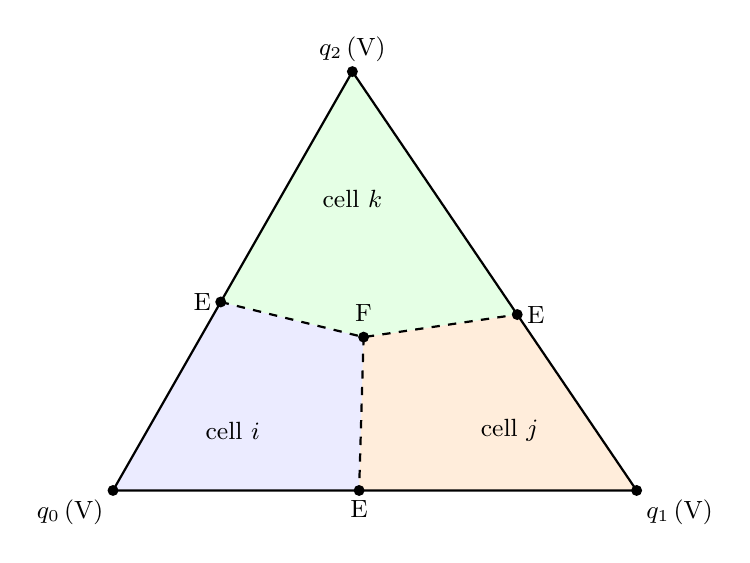
\begin{tikzpicture}[scale=0.95,
    pt/.style={circle, fill, inner sep=1.4pt},
    every node/.style={font=\small}]
  \coordinate (q0) at (0,0);
  \coordinate (q1) at (7,0);
  \coordinate (q2) at (3.2,5.6);
  \coordinate (Eb) at ($(q0)!0.47!(q1)$);
  \coordinate (El) at ($(q0)!0.45!(q2)$);
  \coordinate (Er) at ($(q1)!0.42!(q2)$);
  \coordinate (F)  at (3.35,2.05);
  \fill[blue!8]    (q0) -- (Eb) -- (F) -- (El) -- cycle;
  \fill[orange!14] (q1) -- (Er) -- (F) -- (Eb) -- cycle;
  \fill[green!10]  (q2) -- (El) -- (F) -- (Er) -- cycle;
  \draw[thick] (q0) -- (q1) -- (q2) -- cycle;
  \draw[thick, dashed] (El) -- (F) -- (Er) (F) -- (Eb);
  \foreach \p in {q0,q1,q2,Eb,El,Er,F} \node[pt] at (\p) {};
  \node[below left]  at (q0) {$q_0$\,(V)};
  \node[below right] at (q1) {$q_1$\,(V)};
  \node[above]       at (q2) {$q_2$\,(V)};
  \node[below]       at (Eb) {E};
  \node[left]        at (El) {E};
  \node[right]       at (Er) {E};
  \node[above=2pt]   at (F)  {F};
  \node at (1.6,0.8) {cell $i$};
  \node at (5.3,0.8) {cell $j$};
  \node at (3.2,3.9) {cell $k$};
\end{tikzpicture}
\caption{One triangle of a surface, shared by the cells of seeds $i$, $j$ and $k$. The corners
are \textbf{V} vertices. An \textbf{E} vertex is where a triangle edge crosses a bisector, where
the boundary between two cells (dashed) leaves the triangle. The \textbf{F} vertex is where the
triangle crosses two bisectors at once: where the Voronoi edge of $i$, $j$ and $k$ pierces the
surface. Every F vertex is one triangle $\{i,j,k\}$ of the RDT.}
\label{fig:triangle}
\end{figure}

Cell $i$'s piece of this triangle is the convex polygon $q_0 \to E_\text{bottom} \to F \to
E_\text{left}$: one V, two E and one F. Cell $j$'s is $q_1 \to E_\text{right} \to F \to
E_\text{bottom}$, and cell $k$'s is $q_2 \to E_\text{left} \to F \to E_\text{right}$. Each E is
shared by two cells, and the F by all three. In a \textbf{tet}, or in the box, there is a fourth
kind, C. The table lists all four, with the number of cells each one bounds and the predicate
that tests it against a new bisector (\secref{ssec:family}):

{\small
\begin{xltabular}{\linewidth}{@{}P{0.8cm} L P{1.2cm} P{2.8cm} P{1.6cm}@{}}
\toprule
type & defined by & cells & global key & predicate \\
\midrule
\endhead
\textbf{V} & a domain vertex $q$ (a mesh vertex, a box corner) & 1 & $q$ & \code{side1} \\
\textbf{E} & a domain edge $(q_0, q_1)$ crossing bisector $(i, j)$ & 2 & (edge, $\{i,j\}$)
  & \code{side2} \\
\textbf{F} & a domain face or triangle crossing bisectors $(i,j)$ and $(i,k)$ & 3
  & (face, $\{i,j,k\}$) & \code{side3} \\
\textbf{C} & bisectors $(i,j)$, $(i,k)$, $(i,l)$: a Voronoi vertex & 4 & $\{i,j,k,l\}$
  & \code{side4} \\
\bottomrule
\end{xltabular}}

The \textbf{global key} is the vertex's defining data, normalised: the domain feature it lies on
(a vertex, an edge or a face, and none for C), together with the sorted set of seeds whose
cells it bounds (just the owning cell for V, so the feature alone suffices). It comes out the
same from every cell and every piece that sees the vertex. Four things follow from that:

\begin{enumerate}
\item \textbf{Welding is exact.} Vertices are merged by key in a hash table (\code{mix64}, open
  addressing, as in \code{TetMesh}'s face table). There is no tolerance and no ``merge within
  $10^{-9}$'', and so no cracks and no false merges.
\item \textbf{The dual is free.} Every F key on a surface \emph{is} an RDT triangle
  $\{i,j,k\}$. Every C key in a volume is a Delaunay tet $\{i,j,k,l\}$.
\item \textbf{Validation is combinatorial.} A key of type V, E, F or C must turn up in exactly 1,
  2, 3 or 4 cells, namely those of its seed set. Anything else is a bug you can point at
  (\secref{ssec:consumers}).
\item \textbf{Debugging can answer ``why''.} Click a vertex and the tool can say which seeds and
  which feature made it, and how the predicate that kept it was decided.
\end{enumerate}

Each vertex also carries a \textbf{constructed position} in double, computed from its definition
by a small linear solve. It exists for display and integration only. \textbf{No predicate ever
reads it} (\secref{ssec:rule}).

\subsection{\texorpdfstring{\code{ClippedPolygon}}{ClippedPolygon}: a triangle clipped by one cell}\label{ssec:polygon}

A convex polygon in the triangle's plane, stored as a cycle of (vertex, constraint) pairs, where
constraint $k$ supports the edge from vertex $k$ to vertex $k+1$. It starts as the triangle:
three V vertices and three edge constraints. Clipping by a bisector classifies the vertices. The
vertices on the wrong side form one contiguous run, because the polygon is convex. The run is
replaced by two new vertices: (previous constraint $\cap$ bisector) and (bisector $\cap$ next
constraint). A clipped triangle rarely has more than eight vertices, so it lives in a small
inline buffer that allocates only in the rare case it must grow.

The edges tell you everything else. An edge on bisector $(i,j)$ is a piece of the boundary
between cells $i$ and $j$ on the surface: its length is a facet measure, and $j$ is a neighbour.
An edge on a triangle edge continues into the adjacent triangle, or it is the surface's border.

\subsection{\texorpdfstring{\code{ConvexCell}}{ConvexCell}: a box or tet clipped by one cell, stored as its dual}\label{ssec:convexcell}

This is the structure of \citet{ray2018}, and it is what makes a 3D clipper short enough to
trust. The polytope is stored as:

\begin{itemize}
\item \textbf{planes}: an array of constraints. Six box faces or four tet faces to start with,
  then the bisectors as they cut.
\item \textbf{vertices}: an array of \emph{triangles} $(a, b, c)$, each three indices into the
  planes. A vertex of the polytope is where exactly three planes meet, so it \emph{is} a triangle
  of plane indices: the polytope's dual. Each vertex also carries its symbolic key and its
  constructed position.
\end{itemize}

To \textbf{clip by a plane $P$}: mark the vertices on the wrong side of $P$, using exact
predicates. If none is marked, $P$ does not cut. If all are, the cell is empty. Otherwise the
marked triangles form one patch in the dual, whose boundary is a single cycle of dual edges
$(a,b)$. Add a new triangle $(a, b, P)$ for each boundary edge, and delete the marked ones. That
is the whole operation. Planes that no triangle mentions any more are faces that were cut away.

A concrete case. A cube is 6 planes and 8 triangles: an octahedron in the dual. Cut one corner
off. Its triangle goes, and the three dual edges around the hole each get a new triangle with
$P$. Now it is 7 planes and 10 vertices, and $V - E + F = 10 - 15 + 7 = 2$, as it should be.

Why this and not a half-edge polyhedron:

\begin{itemize}
\item It is \textbf{small}: a Voronoi cell averages 27 vertices, so it fits on the stack.
\item It has \textbf{no pointer bookkeeping} to get wrong.
\item It is \textbf{simple by construction}: symbolic perturbation guarantees that exactly three
  planes meet at each vertex, which is the only thing the representation assumes.
\item \textbf{Every vertex's symbolic definition is its triangle}, for free.
\end{itemize}

A face, for display or integration, is the cycle of triangles around one plane index.

\subsection{\texorpdfstring{\code{NeighbourGraph}}{NeighbourGraph}}\label{ssec:graph}

CSR: $n+1$ offsets and the neighbour ids, each list sorted by id (that is the determinism rule of
\secref{ssec:determinism}). It is symmetric by construction when the predicates are exact, and
validated as such (\secref{ssec:consumers}). Parallel arrays can hang off its entries: the facet
measure and facet centroid, filled by the integrator, which is exactly what the transport
Hessian (\secref{ssec:ot}) and a Laplacian on the seeds need.

\subsection{\texorpdfstring{\code{Generation}}{Generation}: one result, frozen}\label{ssec:generation}

The unit the app publishes. It is immutable and held by \code{shared\_ptr}, and contains
everything needed to show one state: the display meshes, the carrier meshes for overlay
channels, the channel index arrays, per-cell statistics, the validation report, the predicate
counters, and the revisions it was computed from. A computation builds a new one. The host swaps
the pointer between frames, and the viewer keeps the old one alive through
\code{MeshView::keep\_alive} until its layers are gone. \Secref{ssec:generations} has the
details.

% ======================================================================================
\section{Predicates and robustness}\label{sec:predicates}

This section is why the tool can be trusted, and it is also the most interesting part of the
design to look at while it runs.

\subsection{The one rule: predicates read input numbers only}\label{ssec:rule}

Every decision the clippers take is a \emph{predicate}: a question with a yes-or-no answer, such
as ``is this vertex on seed $i$'s side of the bisector of $i$ and $m$?''. The rule is that a
predicate is evaluated from the \textbf{input numbers only}: seed coordinates, weights, and
domain vertex coordinates, exactly as given. It never uses a constructed coordinate, such as the
rounded position of a vertex computed earlier.

Why so strict? A constructed vertex carries rounding error, and two computations that look at the
same vertex through different roundings can disagree. Say cell $i$ decides that the bisector
with $j$ cuts off a sliver of it, while cell $j$ decides that the same facet has zero area. Now
$i$ lists $j$ as a neighbour and $j$ does not list $i$. The tiling has a crack or an overlap. The
dual has a missing triangle. In a propagation, it can loop forever. Floating-point Voronoi codes
live with this through tolerances. This one removes it. Every predicate is the sign of a
polynomial in the input, and the sign of a polynomial in doubles can be computed exactly.

\subsection{The predicate family}\label{ssec:family}

Write
\[
  f_{ia}(x) = \pi_i(x) - \pi_a(x) = 2\,x\cdot(p_a - p_i) - c_a,
  \qquad c_a = \norm{p_a}^2 - \norm{p_i}^2 + w_i - w_a ,
\]
for the difference of power distances. It is an \emph{affine} function of $x$ (the $\norm{x}^2$
cancels, \secref{ssec:halfspaces}): negative on $i$'s side of the bisector of $i$ and $a$,
positive on $a$'s. Each clipping question is ``what is the sign of $f_{im}$ at this vertex?'',
for the cell of seed $i$ and a new bisector $(i, m)$. The vertex types of
\secref{ssec:symbolic} give four predicates:

{\small
\begin{xltabular}{\linewidth}{@{}P{2.9cm} L L@{}}
\toprule
predicate & the vertex it tests & the sign it computes \\
\midrule
\endhead
\code{side1} & a domain vertex $q$ & $f_{im}(q)$. Degree 2 \\
\code{side2} & where the domain edge $(q_0, q_1)$ crosses bisector $(i, j)$
  & a ratio of $2\times 2$ determinants of $f$ values at $q_0$ and $q_1$. Degree 4 over
    degree 2 \\
\code{side3} & where the domain triangle $(q_0, q_1, q_2)$ crosses bisectors $(i,j)$ and $(i,k)$
  & a ratio of $3\times 3$ determinants of $f$ values at the three corners. Degree 6 over
    degree 4 \\
\code{side4} & the Voronoi vertex of $i$, $j$, $k$, $l$
  & the power in-sphere test on the five seeds over \code{orient3d} of four. Degree 5 over
    degree 3 \\
\code{orient3d},\newline \code{in\_power\_sphere} & (not a clipping question)
  & the Delaunay predicates, for the optional Delaunay (\secref{sssec:delaunay}) and for
    validation \\
\bottomrule
\end{xltabular}}

The first three share one shape, and it is worth seeing why. A vertex where $k$ bisectors cross
a $k$-dimensional domain feature (a vertex, an edge or a triangle: $k = 0, 1, 2$) has
barycentric coordinates in that feature. Because every $f_{ia}$ is affine, Cramer's rule turns
``the value of $f_{im}$ at that vertex'' into a ratio of two $(k+1)\times(k+1)$ determinants of
$f$ values at the feature's corners: the denominator has a row of ones, and the numerator has
the row of $f_{im}$ values in its place. Written out,
\begin{align*}
  \text{\code{side1}:}\quad f_{im}(x) &= f_{im}(q),\\[4pt]
  \text{\code{side2}:}\quad f_{im}(x) &=
    \frac{\begin{vmatrix} f_{im}(q_0) & f_{im}(q_1) \\ f_{ij}(q_0) & f_{ij}(q_1) \end{vmatrix}}
         {\begin{vmatrix} 1 & 1 \\ f_{ij}(q_0) & f_{ij}(q_1) \end{vmatrix}},\\[4pt]
  \text{\code{side3}:}\quad f_{im}(x) &=
    \frac{\begin{vmatrix} f_{im}(q_0) & f_{im}(q_1) & f_{im}(q_2) \\
                          f_{ij}(q_0) & f_{ij}(q_1) & f_{ij}(q_2) \\
                          f_{ik}(q_0) & f_{ik}(q_1) & f_{ik}(q_2) \end{vmatrix}}
         {\begin{vmatrix} 1 & 1 & 1 \\
                          f_{ij}(q_0) & f_{ij}(q_1) & f_{ij}(q_2) \\
                          f_{ik}(q_0) & f_{ik}(q_1) & f_{ik}(q_2) \end{vmatrix}},
\end{align*}
and the vertex is on $i$'s side when the ratio is negative. So \code{side1}, \code{side2} and
\code{side3} are one formula at three sizes: one thing to derive, one thing to filter, and one
thing to test. \code{side4} has no domain feature, and comes from solving the three bisector
equations directly. With $u_a = 2\,(p_a - p_i)$ and $c_a$ as above,
\[
  \text{\code{side4}:}\quad f_{im}(x) = -\,
    \frac{\begin{vmatrix} u_j & c_j \\ u_k & c_k \\ u_l & c_l \\ u_m & c_m \end{vmatrix}}
         {\begin{vmatrix} u_j \\ u_k \\ u_l \end{vmatrix}},
\]
where each $u_a$ is a row of three numbers, so the numerator is $4\times 4$ and the denominator
$3\times 3$. The derivations belong in the header of \code{kernel/}, written out in full, in the
style of mesh-dev's \code{winding\_number.h}.

A denominator is never zero for a vertex that the clipper actually created, provided the domain
pieces are not degenerate (\secref{ssec:sos}). Its sign is part of the answer.

\subsection{Fast when easy, exact when not}\label{ssec:filter}

Each predicate is evaluated in up to three steps:

\begin{enumerate}
\item \textbf{Filter.} Evaluate the determinants in double, together with a certified bound on
  their rounding error: a static or semi-static filter, as in \citet{shewchuk1997} and
  \citet{meyer2008}. If a value is farther from zero than its bound, its sign is certain. On
  random input this settles almost every call.
\item \textbf{Exact.} Otherwise evaluate the same polynomials exactly. Start with GMP rationals
  (\code{gmpxx}, already installed here). They are the simplest thing that is obviously
  correct. Shewchuk-style expansion arithmetic is the faster replacement, if profiling on
  degenerate inputs ever says the exact path matters. On random inputs it will not. On a lattice
  it will, because every vertex goes this way.
\item \textbf{Symbolic perturbation}, if the exact value is zero: next section.
\end{enumerate}

\subsection{Ties: symbolic perturbation}\label{ssec:sos}

Imagine every seed's weight increased by an infinitesimal amount $\varepsilon_i$, with
$\varepsilon_0 \gg \varepsilon_1 \gg \varepsilon_2 \gg \cdots$. Seed 0's extra weight is
infinitely larger than seed 1's, which is infinitely larger than seed 2's, and so on, but every
one of them is infinitesimal. This is Simulation of Simplicity \citep{edelsbrunner1990}, in the
spirit of how Geogram's PCK \citep{levy2016} handles the same predicates. Under that imaginary
input, no predicate is ever exactly zero. When the true value is zero, its sign is the sign of
the first non-zero term of its expansion in the $\varepsilon$s, taken in order of priority.

Because perturbing a weight shifts each $f_{ia}$ by a constant ($\varepsilon_a -
\varepsilon_i$), each such term is one of the determinants above with a row replaced by ones: a
smaller predicate of the same family. The chain always ends in a term that cannot be zero. For
\code{side1} that is a comparison of two indices. For the others, the coefficient of the tested
seed's $\varepsilon_m$ is, up to sign, the vertex's own denominator, which is non-zero because
the vertex exists.

What that buys:

\begin{itemize}
\item \textbf{Consistency.} Every predicate answers questions about \emph{the same} imaginary
  input, so all decisions agree with each other, and the output is a valid complex: the diagram
  of the perturbed seeds.
\item \textbf{No special cases in \secref{sec:algorithms}.} A clipper never meets a vertex exactly
  on a plane, and a \code{ConvexCell} vertex always has exactly three planes.
\item \textbf{Honest geometry.} Measures are unaffected, because the perturbation is
  infinitesimal. A cube corner of a cubic lattice, where eight cells meet at one point, becomes
  several ordinary vertices at the same position, joined by zero-length edges, which integrate to
  nothing.
\end{itemize}

Three things to keep in mind:

\begin{itemize}
\item The domain is not perturbed. Degenerate pieces (zero-area triangles, flat tets) are removed
  when the domain is built. They are counted and can be shown, never silently dropped.
\item The tie-break follows the seed index. With Morton order on or off, degenerate inputs get
  different, equally valid combinatorics. The measures are the same either way.
\item A future Delaunay must use the same perturbation, or it will disagree with the clippers
  exactly on degenerate input, which is where agreement is the point.
\end{itemize}

\subsection{The oracle: a second, stupid implementation}\label{ssec:oracle}

For every predicate there is also a reference that does the obvious thing. It constructs the
vertex exactly, in GMP rationals, by solving its defining linear system. Then it compares the
two power distances exactly. There are no determinants to derive, no filters, and no
perturbation: it returns zero on an exact tie. It is slow, and it is correct by inspection.

The tests (\secref{ssec:predtests}) compare every fast predicate to the oracle wherever the
oracle is non-zero, on millions of random and near-degenerate inputs. Where the oracle is zero,
they check the perturbed answer for consistency instead: antisymmetry, and agreement between
predicates about the same vertex. mesh-dev compares its BVH to Geogram's for the same reason:
two implementations built from different starting points should never disagree.

\subsection{Counters and switches}\label{ssec:counters}

Every predicate counts its calls and how each was decided: by the filter, exactly, or by
perturbation. The counters are thread-local and summed at the end. They are integers, so the sum
is deterministic. The app shows them (\secref{ssec:windows}), and two switches go with them:

{\small
\begin{xltabular}{\linewidth}{@{}P{3.1cm} P{4.2cm} L@{}}
\toprule
switch & effect & what it is for \\
\midrule
\endhead
\textbf{exact everywhere} & skip the filter
  & the result must be \emph{bit-identical}. If it is not, a filter is wrong \\
\textbf{floating point only} (unsafe) & filter results trusted even when uncertain, zeros left
  unresolved
  & to see what goes wrong without \secref{sec:predicates}. On a cubic lattice, expect
    asymmetric neighbours and a broken restricted Delaunay triangulation, found by the
    validators and shown in the viewer \\
\bottomrule
\end{xltabular}}

\subsection{Constructions: numbers for looking at, not for deciding}\label{ssec:constructions}

Positions are still needed, to draw the cells and to integrate over them. Each vertex's position
is computed in double from its definition: the barycentric coordinates of the same Cramer
ratios for E and F vertices, and a $3\times 3$ solve for a Voronoi vertex. Integrals are then
accurate to rounding, around $10^{-15}$ relative, which is far below anything a CVT or a
transport solver can see. And a mistake here can only make a picture or an integral slightly
wrong. It can never make the structure inconsistent, because no decision reads these numbers.

% ======================================================================================
\section{Algorithms}\label{sec:algorithms}

\subsection{Stage A: which half-spaces bound each cell}\label{ssec:stageA}

Three neighbour oracles, built in this order. The first is the test reference, the second the
default, and the third an independent second opinion.

\subsubsection{Brute force (the reference)}\label{sssec:brute}

For each seed, start from the box $B$ and clip it by the bisector with \emph{every} other seed.
That is $O(n^2)$, which is useless beyond a few thousand seeds, but it has no stopping rule, no
search structure and no cleverness to be wrong. It is what \secref{sec:testing} compares the
others against.

\subsubsection{Nearest seeds and a security radius (the default)}\label{sssec:meshless}

This is the algorithm of \citet{levy2012} and \citet{ray2018}, made exact. For each seed $i$:

\begin{center}
\fbox{\begin{minipage}{0.9\linewidth}
\begin{enumerate}[label=\arabic*., leftmargin=*]
\item $C \leftarrow$ the box $B$, as a \code{ConvexCell}.
\item For each seed $j \neq i$, nearest first (from the grid, 32 at a time, resumed as needed):
  \begin{enumerate}[label=(\alph*)]
  \item $R \leftarrow$ the largest distance from $p_i$ to a vertex of $C$, rounded up.
  \item If the bisector of $i$ and $j$ lies farther than $R$ from $p_i$: \textbf{stop}. No
    farther seed can cut $C$ either, so the cell is certified.
  \item Clip $C$ by the bisector of $i$ and $j$.
  \end{enumerate}
\item $N(i) \leftarrow$ the seeds whose bisectors are still faces of $C$.
\end{enumerate}
\end{minipage}}
\end{center}

The test in step 2(b) is the one of \secref{ssec:halfspaces}: without weights, stop once
$d_{ij} > 2R$. With weights, replace $w_j$ in $t_{ij}$ by the largest weight in the set. The
resulting bound $(d^2 + w_i - w_{\max})/(2d)$ grows with the distance $d$, so once it exceeds $R$
for the next seed it does so for every farther one, and it can only make the test stop later
than the true weights would, never earlier. $R$ is computed from constructed positions, so it is
enlarged by a margin. \textbf{The certificate may be pessimistic, never optimistic.} Clipping by
one bisector too many costs a little time. Stopping one too early would silently lose a face.
Distance ties are ordered by index, so the order of clipping never depends on anything but the
input.

Why this is the default:

\begin{itemize}
\item It is \textbf{the same code as the RVD}: a \code{ConvexCell} clipped by bisectors. The
  Voronoi maker and the RVD engine are one program from the first day.
\item It is \textbf{embarrassingly parallel}: one seed per task, no shared state.
\item It is \textbf{local}. Any single cell can be computed on its own, typically in
  microseconds, without building anything global. That makes inspecting one cell of a
  ten-million-seed diagram instantaneous, and it is what cell replay (\secref{ssec:replay}) runs
  on.
\item Weights, periodic boxes and anisotropy (\secref{ssec:further}) change only the distance
  order and the certificate, never the structure.
\end{itemize}

Its weak point is strongly non-uniform density, where the grid returns neighbours slowly. That is
the kd-tree's job (\secref{ssec:grid}). With exact predicates the graph comes out symmetric,
$j \in N(i)$ exactly when $i \in N(j)$, even though every cell was computed alone.
Floating-point versions of this algorithm cannot promise that.

\subsubsection{Delaunay (optional, later)}\label{sssec:delaunay}

Incremental Bowyer--Watson, with an infinite vertex for the convex hull, walking point location,
and insertion in biased randomised order over Morton-sorted seeds \citep{amenta2003}. It needs
\code{orient3d} and \code{in\_power\_sphere} with the \textbf{same} perturbation as
\secref{ssec:sos}; \citet{devillers2011} work out perturbations for exactly this case, weighted
Delaunay in 3D. It gives the full, unbounded neighbour graph and every Delaunay tet.

It comes late because it is the largest single piece of code in the project, and nothing in
stages B to D needs it. It comes at all because an independent algorithm for the same graph is
the strongest test there is: restricted to $B$, the Delaunay graph and the meshless graph must be
\emph{identical}, on every input, degenerate ones included. A weighted Delaunay triangulation is
also an output worth having.

\subsection{The 3D clipper}\label{ssec:clipper3d}

The \code{ConvexCell} of \secref{ssec:convexcell} starts from the box, or from a tet. Clipping by
a bisector runs the predicate that matches each vertex's type, and the type is read off the
vertex's three planes:

{\small
\begin{xltabular}{\linewidth}{@{}L P{1.2cm} P{2cm}@{}}
\toprule
the three planes of a vertex & type & predicate \\
\midrule
\endhead
three features (a box corner, a tet vertex)            & V & \code{side1} \\
two features and a bisector (on a domain edge)         & E & \code{side2} \\
one feature and two bisectors (on a domain face)       & F & \code{side3} \\
three bisectors (a Voronoi vertex)                     & C & \code{side4} \\
\bottomrule
\end{xltabular}}

Per cell, the clipper also provides the faces (the cycle of vertices around each plane), $R$ for
the certificate, the volume, the first and second moments (by splitting into tets from one
vertex), and the area and centroid of every bisector face. A clip costs one predicate per vertex,
and a cell has about 27 vertices, so it is a few dozen predicate evaluations per bisector.

\subsection{The polygon clipper}\label{ssec:clipper2d}

The \code{ClippedPolygon} of \secref{ssec:polygon} does the same in a triangle's plane. A
vertex's type is read off its two constraints: two edges make a V, an edge and a bisector an E,
two bisectors an F. It provides the area and moments (from triangles fanned around one vertex),
and the length and midpoint of every bisector edge.

\subsection{Stage B: which pieces each cell meets}\label{ssec:stageB}

This is where Voronoi becomes RVD, and there are two ways to organise it.

{\small
\begin{xltabular}{\linewidth}{@{}P{2.2cm} L L@{}}
\toprule
 & \textbf{cell-centric} (the default) & \textbf{element-centric} (Geogram's way) \\
\midrule
\endhead
outer loop & over seeds & over domain pieces \\
how it finds work
  & ask the AABB tree for the pieces that overlap the bounding box of $V_i \cap B$, and clip each
    one by the bisectors of $N(i)$
  & start from the seed nearest a corner of the piece (nearest in power distance, found by
    walking the neighbour graph from the Euclidean nearest), which owns that corner. Clip, and
    every bisector edge of the result names another cell that also meets the piece. Visit it,
    until none is new \\
complete?
  & always. A piece that meets the cell overlaps its box, however disconnected the restricted
    cell is
  & always. Pieces are convex, so the cells tile each one in a connected pattern \\
output grouped by & seed, so integrals need no reduction
  & piece, so integrals are reduced by seed afterwards \\
parallel over & the $n$ seeds & the pieces \\
best when
  & always good. Essential when seeds outnumber pieces (a cube with 12 triangles and $10^5$
    seeds)
  & pieces outnumber seeds by far, and the pieces that overlap a box but miss the cell cost too
    much \\
\bottomrule
\end{xltabular}}

Build the cell-centric one first. It is complete by an argument you can check in one line, and it
keeps each seed's work in one task. Rejecting a piece that overlaps the box but misses the cell
is cheap: most fail on the first plane, if the planes are tried nearest seed first. The
element-centric traversal is the optimisation to add later if the profile asks for it, and the
two must produce identical results (\secref{ssec:twins}). A third organisation, which validates
each corner of the RVD on its own \citep{sainlot2017}, is worth reading before M8.

\paragraph{The shortcut that makes volumes cheap.} In a volume, most cells never touch the
boundary. If seed $i$ is inside the domain (winding number above one half) and the ball of radius
$R$ around $p_i$ does not reach the boundary surface (\code{nearest\_within} with $R^2$, in
mesh-dev's \code{SurfaceQueries}), then $V_i \cap \Omega$ \emph{is} $V_i \cap B$, and no tet is
needed at all. Only the boundary layer of cells is clipped against tets. This is the same idea as
the clipped Voronoi diagram of \citet{yan2013}, and it makes a volume cost about as much as a
box. The same test against a surface empties the restricted cell of any seed whose ball misses
the surface entirely.

\subsection{Stage C: the consumers}\label{ssec:consumers}

Each consumer receives (seed, piece, clipped polygon or polyhedron) and keeps what it needs.

\paragraph{Mesh builder,} for display and export.
\begin{itemize}
\item On a surface, every clipped polygon is a face. In a volume, a face is kept if it lies on a
  bisector or on the domain boundary. A face on a tet face shared with another tet of the
  \emph{same} cell is internal to the cell and is dropped. Its constraint says so: it is a tet
  face whose neighbouring tet is also in cell $i$.
\item Faces are fanned into triangles. Vertices are welded by symbolic key
  (\secref{ssec:symbolic}), and every triangle records its cell.
\item The adjacency of the restricted cells (cells sharing an arc on a surface, or a face in a
  volume) is coloured greedily, in smallest-last order. When the cells tile a sphere-like
  surface as disks, that graph is planar, and smallest-last greedy never needs more than six
  colours on a planar graph. In a volume it takes more, typically around ten. The triangles are split by
  colour class into one mesh per class, the \emph{chromatic layers} that \secref{ssec:published}
  publishes, and the host gives each class its own colour (the viewer's default palette repeats
  after eight). No two cells that share an arc or a face share a colour.
\item It also builds the \textbf{skeleton}: all welded vertices, the Voronoi edges (polygon edges
  on bisectors, polyhedron edges between two bisector faces), and each vertex's type and how its
  predicate was decided. That is what the overlay channels index.
\end{itemize}

\paragraph{Integrator.} Per seed, the mass, first moment and second moment about $p_i$, with
closed forms on triangles and tets, including a linear density. Per neighbour pair, the facet
measure and centroid. Everything goes into per-seed slots, and totals are
\code{deterministic\_sum}s.

\paragraph{Restricted Delaunay builder.} On a surface, every F key is a triangle $\{i,j,k\}$,
oriented by the domain triangle it was found in. In a volume, every C key is a tet
$\{i,j,k,l\}$, and the F keys on the domain's boundary faces are its boundary triangles. A triple
that appears under two different F keys means a Voronoi edge pierces the surface twice: a
closed-ball violation, and a place where the RDT will fold. It is recorded, not hidden.

\paragraph{Validators,} run from the tests and from a button in the app.

{\small
\begin{xltabular}{\linewidth}{@{}P{2.6cm} L L@{}}
\toprule
check & what must hold & what a failure means \\
\midrule
\endhead
coverage & $\sum_i m_i$ equals the domain's measure, to about $10^{-12}$ relative
  & a hole or overlap in the tiling \\
key census & every V, E, F, C key turns up in exactly 1, 2, 3, 4 cells: those of its seed set
  & an inconsistent predicate, or a clipper bug, located exactly \\
symmetry & $j \in N(i) \iff i \in N(j)$ & a cell computed wrongly on one side \\
facet agreement & the facet $(i,j)$ has the same measure seen from $i$ and from $j$
  & the same, measured \\
nearest-seed sampling & at random points of the domain, the brute-force nearest seed (in power
  distance) is the cell that contains the point & the diagram is not the Voronoi diagram \\
cell topology & each restricted cell is one disk: one component, one boundary loop,
  $\chi = 1$ & the closed ball property fails there (\secref{ssec:closedball}). Not a bug, a
  sampling fact \\
RDT manifoldness & on a closed surface, every RDT edge is in exactly two RDT triangles, and
  $\chi(\text{RDT}) = \chi(S)$ & the remesh is not a valid mesh of $S$ \\
\bottomrule
\end{xltabular}}

Every failure is reported with its indices, so the app can show it as an overlay channel.

\paragraph{Statistics.} Per cell: counts of faces, edges and vertices by type, the mass, and the
dimensionless second moment
\[
  G = \frac{1}{d}\,\frac{\int_{\text{cell}} \norm{x - c}^2\,dx}{\operatorname{vol}^{1+2/d}},
\]
with $c$ the cell's centroid and the density taken as one. It measures a cell's quality
independently of its size: $1/12$ for a cube, and $0.0785$ for the truncated octahedron of the
BCC lattice, the best known in 3D. Histograms go to the panel.

\subsection{Stage D: the optimisers}\label{ssec:optimisers}

Each iteration is one pass of A, B and the integrator, and each iteration can become a
generation for the viewer (\secref{ssec:generations}), so every optimiser can be watched.

\begin{itemize}
\item \textbf{Lloyd.} $p_i \leftarrow c_i$. On a surface, optionally move $c_i$ to the nearest
  point of the surface, from mesh-dev's BVH (\secref{ssec:integrals}). The energy is recorded at
  every step. Stop when its relative decrease, or the largest step measured in cell sizes, falls
  below a tolerance.
\item \textbf{L-BFGS} on the CVT energy, with gradient $2\,m_i\,(p_i - c_i)$, using
  \code{lbfgs-lite} from mesh-dev. Every line-search trial is one more pass. On a surface, the
  gradient is projected onto the tangent planes and the positions back onto the surface.
\item \textbf{Newton on the weights} for transport. Masses and facet measures give the gradient
  and the graph-Laplacian Hessian of \secref{ssec:ot}. Solve with Eigen: conjugate gradients with
  a Jacobi preconditioner, or a sparse $LDL^\mathsf{T}$ at moderate sizes. Fix one weight,
  because shifting every weight by the same amount changes nothing. Damp the step so that no
  cell's mass falls below a floor, the safeguard of \citet{kitagawa2019}. Stop when the largest
  $\lvert m_i - \nu_i\rvert$ is below a tolerance.
\end{itemize}

% ======================================================================================
\section{On top of mesh-viewer}\label{sec:viewer}

The viewer needs no change for anything before milestone M6 (\secref{sec:plan}). This section
maps the design onto its actual interfaces: \code{MeshSource}, \code{OverlaySource},
\code{Panel}, \code{defer}, revisions and \code{keep\_alive}. Two small, general extensions for
later are in \secref{ssec:extensions}.

\subsection{The host, in the viewer's own terms}\label{ssec:host}

It follows the ``Writing a host'' part of the viewer's README, and \code{examples/demo.cpp} is the
template.

\begin{itemize}
\item \textbf{\code{RvdSession}} (core side, no GL) owns the domain, the seeds, the parameters and
  the current generation. It is the counterpart of mesh-dev's \code{Document}.
\item \textbf{\code{RvdSource}}, a \code{MeshSource}, and \textbf{\code{RvdOverlay}}, an
  \code{OverlaySource}, are thin adapters over the current generation, the counterpart of mesh-dev's
  \code{document\_source.h}. Nothing is copied: a \code{MeshView} points into the generation's
  arrays.
\item \textbf{Panels} hold the controls (\secref{ssec:windows}).
\item \code{main} declares the session before the viewer, so it outlives the GPU copies. A dropped
  \code{.obj} or \code{.msh} becomes the domain, and a dropped point file becomes the seeds,
  through \code{set\_drop\_handler}.
\end{itemize}

\subsection{What is published}\label{ssec:published}

{\small
\begin{xltabular}{\linewidth}{@{}P{2.2cm} L L@{}}
\toprule
mesh & what it holds & why it is shaped like this \\
\midrule
\endhead
\textbf{domain}
  & the domain's vertices, and its surface triangles, or a volume's hull and its tets, or the
    box's 12 triangles. Stable id; the revision changes when the domain moves
  & \textbf{listed first}: the first mesh fixes the scene origin, and \code{mesh\_center} reads
    triangles only, so a points-only mesh first would put the origin at zero. On a surface the
    host hides it while cells are shown, because the cells lie exactly on it and two coplanar
    layers z-fight \\
\textbf{seeds}
  & the seed positions, and no triangles. Stable id; the revision changes whenever the seeds
    move, every Lloyd step
  & a \emph{carrier}: it draws nothing, and holds the vertices the seed channels index.
    \code{closed~=~false} \\
\textbf{cells, class $k$} (for $k < K$)
  & the vertices of that class's cells, copied per cell, and the faces of those cells. A new id
    per generation; the revision changes when the shrink slider moves
  & one colour per layer, so one layer per colour class (\secref{ssec:consumers}). Copies per
    cell make ``shrink cells toward their centroid'' a position-only change: interactive, with no
    new ids. In 3D, \code{closed~=~true} and \code{oriented~=~true} (faces wound outward): each
    layer is a union of closed polyhedra, so the viewer's stencil cap fills every cut cell's
    cross-section in a shade of its class colour, for free \\
\textbf{skeleton}
  & the welded vertices of the whole diagram, and no triangles. A new id per generation
  & the carrier for the Voronoi edges and every vertex channel. A channel indexes one mesh, and
    the edges between two classes belong to neither class layer \\
\textbf{RDT}
  & the generation's snapshot of the seed positions, and the RDT triangles; in a volume, the RDT
    tets (positively oriented) and their hull. A new id per generation
  & the remesh, in \emph{shaded + edges} mode. In a volume, the viewer's cutting plane shows the
    Delaunay tets standing in the cut, and \code{tet\_labels} can mark slivers, so
    \textbf{by label} colours them \\
\textbf{inspector}
  & an icosphere, a quad, and the replayed cell. The first two have stable ids and new positions
    when the selection changes; the replayed cell gets a new id per step
  & the security sphere, the bisector being clipped, and the partial cell of
    \secref{ssec:replay} \\
\bottomrule
\end{xltabular}}

\subsection{Overlay channels}\label{ssec:channels}

A fixed list, always present, emptied rather than removed. The viewer keeps a channel's colour
and checkbox while the same name stays in the same slot, so a stable order is what makes the
user's settings survive every run. This is mesh-dev's \code{DebugDraw::reset} rule.

{\small
\begin{xltabular}{\linewidth}{@{}P{3.3cm} P{1.5cm} P{1.6cm} L@{}}
\toprule
channel & primitive & indexes & shows \\
\midrule
\endhead
seeds                   & points & seeds    & every seed \\
selection               & points & seeds    & the selected seed and its neighbours \\
neighbour graph         & lines  & seeds    & the pairs $(i,j)$, $i<j$: the Delaunay edges whose
                                              Voronoi facet meets $B$ \\
Voronoi edges           & lines  & skeleton & the diagram's edges, which the fanned triangles'
                                              own edges would clutter \\
decided exactly         & points & skeleton & vertices where a filter was not enough: the
                                              robustness microscope \\
decided by perturbation & points & skeleton & vertices that exist only thanks to
                                              \secref{ssec:sos}, where the input is degenerate \\
closed-ball violations  & points & skeleton & cells that are not disks, pairs sharing two arcs,
                                              Voronoi edges piercing twice \\
validator failures      & points & skeleton & should be empty, always. Any point here is a bug
                                              with an address \\
\bottomrule
\end{xltabular}}

Channels draw even when their layer is hidden, and \textbf{in front} lifts them over opaque
cells, which is exactly what the seed and skeleton carriers need.

\subsection{Generations, ids, and keeping what the user set}\label{ssec:generations}

The viewer uploads a mesh's triangles once, the first time it sees its id, and a host must never
reuse an id. A new diagram has new connectivity, so it gets new ids from a counter in the host.
Each generation is an immutable object, and every \code{MeshView} from it carries
\code{keep\_alive}, the generation's \code{shared\_ptr}. The viewer then holds the generation for
as long as any layer shows it, and there is no destruction order to think about.

A new id is a new \code{Layer}, with default colour, alpha and visibility. Left alone, every
Lloyd step would undo what the user set in the View window. So the host \textbf{carries the style
over} when it installs a generation:

\begin{enumerate}
\item read each outgoing layer's settings through \code{viewer.scene().layer(old\_id)}: colour,
  alpha, visibility, cap and solid cap;
\item swap in the new generation;
\item call \code{viewer.sync()}, which is public, so the new layers exist now rather than at the
  end of the frame;
\item write the settings into \code{viewer.scene().layer(new\_id)}, with class $k$ inheriting from
  class $k$.
\end{enumerate}

The first time a class layer appears there is nothing to inherit. The host then gives it its
class colour and turns its \textbf{cap} on, which the viewer leaves off by default. That is what
makes a cut through 3D cells read as a section of solid cells rather than of hollow shells.

One thing this cannot keep is a custom \textbf{composite order}: \code{Scene::sync} rebuilds the
order from scratch when a layer disappears. So in phase one the source lists its meshes in the
order that composites best, and the topology revision of \secref{ssec:extensions} is the real
fix.

The one mutable thing is \textbf{display positions}. The class layers' positions are a host-owned
array derived from the generation, with each cell scaled toward its centroid by the shrink
factor. Moving the slider rewrites that array and bumps the revision: same ids, no new
generation, and the viewer re-uploads positions only.

\subsection{The frame, and where the work happens}\label{ssec:frame}

The viewer's frame order decides where each kind of work goes.

{\small
\begin{xltabular}{\linewidth}{@{}P{5.4cm} L@{}}
\toprule
the viewer's frame, in order & what RVD does there \\
\midrule
\endhead
wait for input, or poll while a panel is \code{animating()} & \\
ImGui frame: each open window's \code{Panel::ui}
  & widgets and parameters only. A button calls \code{viewer.defer(compute)}, and never
    computes \\
run what the panels deferred & a one-off run: A, B, C, and a new generation \\
\code{Panel::update} on every panel
  & a running optimiser: one iteration per frame (or a time budget), then the new generation
    and the style carry-over of \secref{ssec:generations} \\
\code{Scene::sync}, then the overlay's & new layers appear, old ones go \\
\code{Renderer::draw} & \\
\bottomrule
\end{xltabular}}

\begin{itemize}
\item \textbf{One-off runs} are deferred, so they never run inside an open ImGui window and never
  change the meshes halfway through drawing the windows that describe them. That is the viewer's
  own rule, from \code{viewer.h}.
\item \textbf{Optimisers} step in \code{update} and return \code{animating()~==~true} while
  running, so the viewer polls instead of sleeping. A Lloyd loop is a clock, like the demo's
  wobble.
\item \textbf{Big diagrams} go to a worker thread. It snapshots the seeds, computes a generation,
  and \code{update} swaps it in when it is ready, while the viewer keeps drawing the last one.
  Generations are immutable, so nothing is shared mutably across threads. A cancel flag is
  checked between seeds.
\end{itemize}

\subsection{Windows}\label{ssec:windows}

Four panels:

{\small
\begin{xltabular}{\linewidth}{@{}P{2.2cm} L@{}}
\toprule
window & contents \\
\midrule
\endhead
\textbf{Diagram}
  & the domain (box, surface, volume; from a file or a generator). The seeds (count, sampler,
    random seed, weights). The neighbour oracle (brute force, meshless, Delaunay) and the
    traversal (cell- or element-centric). The display (shrink, classes, skeleton).
    \textbf{run} \\
\textbf{Optimise}
  & Lloyd, L-BFGS or transport. Iterations per frame. Live plots of the energy and the gradient
    norm (\code{ImGui::PlotLines}). Start and stop \\
\textbf{Cell}
  & the selected cell: seed, weight, mass, centroid, $G$, counts by vertex type, and its
    neighbours as buttons that select them. The replay controls (\secref{ssec:replay}). The
    security sphere \\
\textbf{Robustness}
  & predicate counters per predicate and per decision path. The two switches of
    \secref{ssec:counters}. \textbf{validate}, with each failure listed next to the channel
    that shows it. The closed-ball summary \\
\bottomrule
\end{xltabular}}

Keys: the viewer owns Esc, F, W and P. The host takes \textbf{C} (select the cell under the
cursor), \textbf{[} and \textbf{]} (replay one clip back or forward), and \textbf{L} (start or
stop the optimiser).

\subsection{Picking a cell}\label{ssec:picking}

The viewer has no click hook for hosts, but everything needed is public. On \textbf{C}, read the
mouse position from ImGui's IO. It is in window units, so multiply by
\code{DisplayFramebufferScale} to get the framebuffer pixels the camera works in, then call
\code{Camera::screen\_ray}. The ray is in \emph{scene} space, so add \code{Scene::origin()} to
get file space. Intersect it with the class layers' triangles, skipping hidden layers and hits on
the clipped side of the cutting plane. Brute force is fine for one click, even over millions of
triangles. The hit triangle's cell id is the selection.

\subsection{Where the viewer pinches, and two small extensions}\label{ssec:extensions}

Phase one lives with four things:

\begin{enumerate}
\item \textbf{One colour per layer}, hence the chromatic layers.
\item \textbf{Connectivity fixed per id}, hence new ids per generation, the style carry-over, and
  a composite order that resets.
\item \textbf{No click hook for hosts}, hence picking on a key.
\item \textbf{Label colours only for tets in the cut}, not for triangles.
\end{enumerate}

Two extensions would remove the first two. Both are general, not specific to RVD, and both keep
the viewer's ``positions only'' vertex layout:

\begin{itemize}
\item \textbf{(a) Per-triangle labels.} \code{MeshView} gains one small integer per drawn
  triangle, under the existing \code{labels\_revision}. The surface shader looks the label up by
  \code{gl\_PrimitiveID} in a texture buffer, both core in GL~3.3, and takes its colour from the
  layer's \code{LabelStyle} list, editable in Inspect as tet labels already are. Then one layer
  carries the whole diagram, coloured per cell class or per anything: materials, patches, a
  segmentation in mesh-dev.
\item \textbf{(b) A topology revision.} \code{MeshView} gains a \code{topology\_revision}. When it
  changes, \code{Layer::refresh} re-uploads the index buffer and re-derives the drawn vertices,
  but keeps the layer, its settings and its place in the composite order. That removes the id
  churn and the carry-over code, and helps any host that remeshes.
\end{itemize}

Neither is required before M6, and both are small enough to review in one sitting. A click hook
(\code{Panel::on\_click} with a scene-space ray) is the third candidate, with the lowest
priority.

% ======================================================================================
\section{Implementation plan}\label{sec:plan}

Ten milestones, in order. Every one ends with a test suite that proves it and a picture that
shows it. Nothing is built before the thing that checks it.

\newcommand{\milestone}[1]{\subsection*{#1}\addcontentsline{toc}{subsection}{#1}}

\milestone{M0.\ The skeleton}
\begin{itemize}
\item CMake with \code{rvd\_core}, \code{rvd} and the test binaries. \code{ext/mesh-viewer} as a
  submodule. The \code{RVD\_MESH\_DEV\_DIR} option (\secref{ssec:reuse}).
  \code{-DRVD\_BUILD\_VIEWER=OFF} for headless machines.
\item The host: an \code{RvdSession}, the two sources, the four empty windows. A box domain and
  uniform random seeds, regenerated by a deferred button.
\item \textbf{Done when} the app shows a box with a point cloud in it, and \code{ctest} runs an
  empty suite with no display.
\end{itemize}

\milestone{M1.\ Predicates}
\begin{itemize}
\item \code{kernel/}: \code{side1} to \code{side4}, \code{orient3d}, \code{in\_power\_sphere},
  each filtered, exact with GMP, and perturbed (\secref{sec:predicates}). The oracle. The
  counters.
\item \textbf{Tests:} \code{predicates} (\secref{ssec:predtests}).
\item \textbf{Done when} millions of random and near-degenerate cases agree with the oracle, and
  the perturbed answers pass the consistency checks. You will see nothing new yet, and that is
  right: this is the foundation, and it is proven before anything stands on it.
\end{itemize}

\milestone{M2.\ One cell, then all of them the slow way}
\begin{itemize}
\item \code{ConvexCell} (\secref{ssec:convexcell}): from a box, clip, faces, moments. The
  brute-force oracle (\secref{sssec:brute}) for every seed. The mesh builder with chromatic
  layers, the skeleton, the Voronoi-edges channel, the \textbf{Cell} window.
\item \textbf{Tests:} \code{convex\_cell} (a cube's corner cut, a tet, hand-checked cuts), and
  \code{voronoi\_box} (\secref{ssec:invariants}, with the lattices of \secref{ssec:known}).
\item \textbf{You see} the first Voronoi diagram: coloured cells, cut open by the plane with their
  cross-sections capped. Then the cubic lattice, where every vertex needs \secref{ssec:sos}, and
  the Kelvin cells of the BCC lattice.
\end{itemize}

\milestone{M3.\ Fast Voronoi in a box}
\begin{itemize}
\item The grid (\secref{ssec:grid}), the security radius (\secref{sssec:meshless}), OpenMP over
  seeds, and the deterministic collection of results.
\item \textbf{Tests:} meshless against brute force (\secref{ssec:twins}), the Meijering
  statistics (\secref{ssec:known}), thread independence (\secref{ssec:determinismtest}), and the
  first benchmark (\secref{ssec:bench}).
\item \textbf{You see} a diagram of $10^5$ seeds drawn whole, a $10^6$-seed one computed and
  inspected cell by cell (drawn whole it would be tens of millions of triangles, too many for a
  laptop GPU), the Robustness window's counters, and cell replay.
\end{itemize}

\milestone{M4.\ Restricted to a surface}
\begin{itemize}
\item \code{SurfaceDomain} over mesh-dev's \code{SurfaceMesh}. The \code{ClippedPolygon}
  (\secref{ssec:polygon}). The cell-centric traversal with its AABB tree (\secref{ssec:stageB}).
  The RDT builder, and the closed-ball checks.
\item \textbf{Tests:} \code{rvd\_surface} (\secref{ssec:invariants} and \secref{ssec:known}):
  coverage, key census, nearest-seed sampling, the flat square against the box, the sphere and
  the torus, the thin plate.
\item \textbf{You see} a surface tiled by coloured patches, its remesh, and the closed-ball
  violations lighting up wherever the sampling is too coarse. This is the milestone where the
  tool starts doing something no other one shows you.
\end{itemize}

\milestone{M5.\ Integration and Lloyd}
\begin{itemize}
\item The integrator with a density, Lloyd, then L-BFGS (\secref{ssec:optimisers}). The energy
  plot, and stepping live.
\item \textbf{Tests:} the gradient against finite differences, Lloyd's monotone energy, and the
  second moment of the hexagonal lattice on a flat surface (\secref{ssec:known}), which checks the
  surface integrals.
\item \textbf{You see} isotropic remeshing happen: a random sampling of a surface relaxing, frame
  by frame, into nearly hexagonal cells.
\end{itemize}

\milestone{M6.\ Restricted to a volume}
\begin{itemize}
\item \code{VolumeDomain} over mesh-dev's \code{TetMesh}. The interior-cell shortcut through the
  winding number (\secref{ssec:stageB}). RDT tets. Viewer extension (b) of
  \secref{ssec:extensions}, if the carry-over has become annoying by then.
\item \textbf{Tests:} a box as a tet mesh against the box itself, an L-shaped domain, a sphere,
  coverage.
\item \textbf{You see} cells clipped by a curved volume, capped where the plane cuts them, and the
  Delaunay tets of the clipped diagram standing in the cut.
\end{itemize}

\milestone{M7.\ Weights and transport}
\begin{itemize}
\item Weights through every stage (the predicates have had them since M1). The weighted
  certificate. Newton on the weights.
\item \textbf{Tests:} target masses reached to tolerance, the Hessian against finite differences,
  empty cells handled rather than fatal.
\item \textbf{You see} cells trading volume until every one has its share, live.
\end{itemize}

\milestone{M8.\ Speed and second opinions}
\begin{itemize}
\item The element-centric traversal, the kd-tree, the Delaunay of \secref{sssec:delaunay}, and an
  optional comparison against Geogram in the style of \code{bench\_vs\_geogram.cpp}.
\item \textbf{Tests:} everything above, passed by the new code paths as well, and identical
  results between the paths.
\end{itemize}

\milestone{M9.\ Outward}
\begin{itemize}
\item Writers: \code{.obj} with a group per cell, \code{.msh} with the cell id as element data (so
  Gmsh shows it), and \code{.csv} of per-cell statistics. A Python module over pybind11, numpy in
  and numpy out, the way mesh-dev's is.
\end{itemize}

% ======================================================================================
\section{Testing}\label{sec:testing}

\subsection{The harness}\label{ssec:harness}

mesh-dev's own: one source file per suite, \code{check()} and \code{report\_checks()} from
\code{test\_support.h}, quiet when passing, registered with \code{ctest}. Every random generator
has a fixed seed. \textbf{Every diagram built in any test also runs every validator of
\secref{ssec:consumers}}, so an invariant is checked hundreds of times on inputs nobody designed
to break it, not once on a picked example.

\subsection{Predicates against the oracle}\label{ssec:predtests}

\begin{itemize}
\item \textbf{Random inputs}, uniform in a unit box, and the same shifted by $10^6$ so that the
  cancellation is severe. Every fast predicate must agree with the GMP oracle of
  \secref{ssec:oracle} wherever the oracle is non-zero.
\item \textbf{Near-degenerate inputs}, made from exact degenerate ones. Integer points on a
  sphere ($x^2 + y^2 + z^2 = r^2$ has many integer solutions) give five exactly cospherical
  seeds, and moving one coordinate by an ulp gives the hardest cases a filter can meet. Lattices
  and mirrored seed pairs give degenerate \code{side1} to \code{side3}, with domain vertices on
  bisectors.
\item \textbf{Perturbation consistency} where the oracle says zero: \code{side1} is antisymmetric
  in its two seeds; the filtered and exact paths return the same perturbed sign; and the
  predicates that describe one vertex from different pieces agree about it.
\end{itemize}

\subsection{Invariants, on everything}\label{ssec:invariants}

The validator table of \secref{ssec:consumers} is the core of every diagram test: coverage, key
census, neighbour symmetry, facet agreement, and nearest-seed sampling. They run on random seeds,
on clustered seeds, on seeds outside the domain, and on every input of \secref{ssec:known}.

\subsection{Known answers}\label{ssec:known}

The part that is fun to watch pass. Every row is a closed-form fact the engine must reproduce.
The second moments are those of \citet{conway1999}, and $G$ is defined in
\secref{ssec:consumers}.

{\small
\begin{xltabular}{\linewidth}{@{}P{4.4cm} L@{}}
\toprule
input & what must come out \\
\midrule
\endhead
cubic lattice, box aligned with the cells
  & every cell a cube: 6 faces of non-zero area, $G = 1/12$ to rounding. Every vertex needs
    \secref{ssec:sos} \\
BCC lattice, interior cells
  & the truncated octahedron (Kelvin's cell): 14 faces (6 squares, 8 hexagons), 24 vertices,
    $G = 0.0785433$. Fully generic, so the counts are exact \\
FCC lattice, interior cells
  & the rhombic dodecahedron: 12 faces of non-zero area, $G = 0.0787451$. Six of its vertices
    are where four faces meet, so perturbation splits them: count after merging zero-length
    edges \\
uniform random seeds, cells away from the box
  & mean faces $\to 48\pi^2/35 + 2 \approx 15.54$, mean vertices $\to 96\pi^2/35 \approx 27.07$
    \citep{meijering1953} \\
hexagonal lattice on a flat surface
  & regular hexagons, $G = 5/(36\sqrt{3}) \approx 0.0801875$: the surface path reproducing a 2D
    fact \\
seeds on a plane, a flat square as the domain
  & the surface RVD equals the 2D Voronoi diagram, which is also the box diagram of a thin slab
    around the plane, sliced: its cells are prisms \\
sphere, sampling fine enough
  & a valid RDT, $\chi = 2$. With $n$ the seeds whose restricted cell is non-empty, the
    restricted neighbour counts (cells sharing an arc on the surface) sum to exactly $6n - 12$ \\
torus, sampling fine enough
  & $\chi = 0$, and the restricted neighbour counts sum to exactly $6n$ \\
seeds all on one sphere, in a box around it
  & every cell a cone from the centre, clipped by the box. The centre is a vertex of \emph{all}
    $n$ cells: the worst perturbation test there is \\
duplicate seeds
  & the later duplicate's cell is empty, and the count is reported \\
thin plate, a few seeds on one face only
  & every restricted cell reaches through to the other face: two components each, both
    found \\
\bottomrule
\end{xltabular}}

\subsection{Two ways, one answer}\label{ssec:twins}

Every algorithm has a twin, and twins must agree.

{\small
\begin{xltabular}{\linewidth}{@{}P{5.6cm} L@{}}
\toprule
pair & must agree on \\
\midrule
\endhead
brute force and meshless (\secref{ssec:stageA})
  & the neighbour graph and the key sets, exactly; measures to $10^{-14}$ relative (the clipping
    order differs, so sums round differently) \\
cell-centric and element-centric (\secref{ssec:stageB}) & everything \\
a box domain, and the same box as a tet mesh
  & every cell's neighbours exactly, and its volume and centroid to rounding \\
filtered, and exact everywhere (\secref{ssec:counters}) & everything, \textbf{bit for bit} \\
meshless and Delaunay (M8)
  & the neighbour graph inside $B$, exactly, degenerate inputs included \\
\bottomrule
\end{xltabular}}

\subsection{Optimisers}\label{ssec:opttests}

\begin{itemize}
\item The CVT gradient against central finite differences, at generic configurations, where the
  energy is smooth.
\item Lloyd's energy never increases: with seeds free in space, and with seeds moved to the true
  nearest point of a surface (\secref{ssec:integrals}).
\item L-BFGS reaches a lower energy than Lloyd in fewer passes.
\item Transport: masses within tolerance, and the Laplacian Hessian against finite differences of
  the masses.
\end{itemize}

\subsection{Against Geogram (optional)}\label{ssec:geogram}

A separate target, off unless pointed at a Geogram tree, exactly like \code{MESH\_DEV\_GEOGRAM\_ROOT}
in mesh-dev. I found no Geogram installation on this machine, so it would have to be built
first. Same seeds, same surface: the cell areas agree to rounding, and on generic inputs the sets
of RDT triangles are identical. On degenerate inputs the two perturbation schemes may
legitimately differ, so only measures are compared there.

\subsection{Determinism}\label{ssec:determinismtest}

The same diagram on 1, 2 and 8 threads, and twice in a row: one hash over every output array must
be identical. This is the RVD version of mesh-dev's \code{bench\_pipeline.py -{}-compare} rule.

\subsection{Benchmarks}\label{ssec:bench}

Timings per stage, with the predicate decision paths printed next to them, so that a slowdown can
be traced to the filter:

\begin{itemize}
\item the box: $10^4$, $10^5$ and $10^6$ seeds, uniform and clustered;
\item a sphere of $10^4$ triangles with $10^3$ to $10^5$ seeds, and a fine surface of $10^6$
  triangles with $10^4$ seeds (both regimes of \secref{ssec:stageB});
\item a volume, with and without the interior-cell shortcut.
\end{itemize}

Timing on the laptop is noisy by up to a factor of two, as mesh-dev's notes say, so compare
best-of-$N$ runs, back to back.

\subsection{The gallery}\label{ssec:gallery}

Every input of \secref{ssec:known} is also a menu entry in the Diagram window. They are not
automated tests, but they are where you look first when something is off, and the fastest way to
show someone what the tool does.

% ======================================================================================
\section{From a Voronoi diagram to a restricted one}\label{sec:generalisation}

This is the question you asked, so here is the direct answer.

\subsection{The short version}\label{ssec:short}

The plain Voronoi maker is stage A and stage B run on a domain with one piece, the box. The RVD
adds domains with many pieces, a clipper for flat pieces, and a traversal that picks the pieces
near each cell. It rewrites nothing. The predicates it needs with domain features (\code{side2}
and \code{side3}) are already needed by the box, whose edges and faces are domain features too.
So by the time the box works \emph{exactly}, most of the RVD's difficulty is already solved.

{\small
\begin{xltabular}{\linewidth}{@{}P{2.3cm} L L L@{}}
\toprule
concern & Voronoi in a box & RVD on a surface & RVD in a volume \\
\midrule
\endhead
domain pieces & 1, the box & triangles & tets \\
clipper & \code{ConvexCell} from a box & \code{ClippedPolygon} from a triangle
  & \code{ConvexCell} from a tet \\
vertex types & V (corners), E (box edges), F (box faces), C & V, E, F & V, E, F, C \\
predicates & \code{side1} to \code{side4} & \code{side1} to \code{side3}
  & \code{side1} to \code{side4} \\
traversal & none needed: one piece & cell-centric, with the AABB tree
  & the same, plus the interior-cell shortcut \\
welding keys & seeds and box features & seeds, mesh edges and triangles
  & seeds, mesh edges and faces \\
the dual & Delaunay tets whose Voronoi vertex lies in $B$ & RDT triangles & RDT tets \\
integrals & volumes and moments & areas and moments & volumes and moments \\
\bottomrule
\end{xltabular}}

\subsection{The rules that keep the step small}\label{ssec:rules}

These are what to hold on to while building the Voronoi part, because each one is cheap on day
one and expensive to retrofit:

\begin{enumerate}
\item \textbf{The box is a domain from the first line.} Its corners, edges and faces are features
  with ids, and the vertices on them are symbolic V, E and F vertices. They are not
  floating-point intersections of six planes.
\item \textbf{Always stream (seed, piece, clipped piece)}, even when there is only one piece. No
  consumer is ever allowed to assume that a cell is a single convex piece.
\item \textbf{Predicates talk about domain vertices}, never about planes computed from them. That
  keeps the degrees low, and it is what \code{side2} and \code{side3} will need on triangles and
  tets.
\item \textbf{Weights from day one}, zero by default.
\item \textbf{Stage A always clips the domain's bounding box $B$.} The restricted case needs
  exactly that, and nothing more.
\item \textbf{Write the surface arithmetic in dot products}, so that lifting to $\R^d$ later
  (\secref{ssec:further}) is a change of vector type, not of algorithm.
\end{enumerate}

\subsection{Further, in order of effort}\label{ssec:further}

{\small
\begin{xltabular}{\linewidth}{@{}P{3.2cm} L P{3.3cm}@{}}
\toprule
generalisation & what changes & effort \\
\midrule
\endhead
power (Laguerre) diagrams & weights in $f_{ij}$, and the certificate uses the largest weight
  & already in the design \\
a density & linear $\rho$ on every piece, closed-form integrals & already in the design \\
restricted to curves (boundary curves, feature lines)
  & segments as pieces, a segment clipper, vertex types V and E, predicates \code{side1} and
    \code{side2} & small \\
labelled volumes (materials, inside and outside)
  & tets carry a label, restricted cells are split per (seed, label), and interfaces become
    facets of their own & small, and the bridge to mesh-dev's labelled domains \\
periodic box
  & the distance order and the bisectors use translated images of the seeds, and keys carry the
    image offset & moderate \\
anisotropic, on surfaces
  & lift the surface and the seeds to $\R^6$, as $(x, s\,n)$, the way the VorPaLine method of
    \citet{levy2012} does. The surface clipper and \code{side1} to \code{side3} are dot
    products, so they work in any dimension & moderate, if rule 6 was kept \\
geodesic Voronoi on a surface & bisectors are no longer planes & a different project \\
Apollonius, or multiplicatively weighted & bisectors are hyperboloids or spheres
  & out of scope \\
\bottomrule
\end{xltabular}}

\subsection{Where it could meet your own work}\label{ssec:yourwork}

These are possibilities for you to judge, not claims:

\begin{itemize}
\item \textbf{CVT remeshing of a target surface}, such as a bubble's interface, gives nearly
  regular triangles with density control, as an RDT. That is an alternative, or a complement, to
  remeshing it elsewhere.
\item \textbf{A Voronoi diagram clipped by the interface} gives each cell's volume inside and
  outside the bubble: a volume fraction per cell, computed exactly rather than by sampling. You
  already have the winding numbers and the inside and outside labels.
\item \textbf{Constant-volume Lagrangian cells} through transport \citep{degoes2015,levy2022} are
  a different discretisation of two-phase flow, and expensive to explore without exactly this
  kind of tool.
\item \textbf{Point placement} for any mesh you seed, with the quality of every cell measured.
\end{itemize}

% ======================================================================================
\section{What makes this worth building}\label{sec:interesting}

You said you cannot find good RVD software. The features below are the ones I have not seen in
any of it. Each one is cheap \emph{only because} of the decisions of \secref{sec:idea}: symbolic
vertices, exact predicates with counters, streamed pieces, and a viewer you own.

\subsection{A robustness microscope}\label{ssec:microscope}

Every vertex remembers how its existence was decided: by the filter, by exact arithmetic, or by
perturbation. Two overlay channels show the last two, and the Robustness window counts all three
per predicate. Look at random seeds and a handful of points light up. Look at a cubic lattice and
every vertex does. Look at a symmetric part seeded symmetrically, and exactly its mirror planes
light up, because that is where mesh vertices sit on bisectors. You see where your input is
degenerate before it bites you somewhere else. Flip to \emph{floating point only} and the
validators show you what exact arithmetic was protecting: asymmetric neighbours, cracks in the
coverage, a folded RDT, each with an address.

\subsection{A closed-ball inspector}\label{ssec:closedball}

The closed ball property of \secref{ssec:rdt} is the exact condition for the restricted Delaunay
triangulation to be a valid mesh of the surface. The validators test every clause of it:

\begin{itemize}
\item each restricted cell is one disk;
\item each pair of cells shares at most one arc;
\item each Voronoi edge pierces the surface at most once.
\end{itemize}

Every violation becomes a point in a channel. That is precisely the map of where the sampling is
too coarse for the surface's features: thin parts, sharp creases, close sheets. It also suggests
an experiment no existing tool makes easy. Insert a seed at each violation, at the point of the
offending cell farthest from its seed, in the spirit of the refinement of
\citet{boissonnat2005}. Relax with a few CVT steps and repeat until nothing lights up. The result
is a CVT remesh that is valid by the theorem, not just by looking right.

\subsection{Cell replay, and ``why does this vertex exist?''}\label{ssec:replay}

Select a cell, then step through its construction one bisector at a time with \textbf{[} and
\textbf{]}. At each step the viewer shows the partial polytope, the bisector plane that cuts it
next, the security sphere, and the distance to the next neighbour, and you watch the certificate
fire. On a surface, the same works for one triangle being cut up by the cells that meet it.
Select a vertex and the Cell window says what it is. For example: ``F vertex on triangle 812,
seeds 4, 17 and 23; \code{side3} decided by the filter; constructed at (\dots)''. This is the
debugger you would want on the day a result looks wrong, and it comes from stage A being local
(\secref{sssec:meshless}).

\subsection{Optimisation you can watch}\label{ssec:watch}

Lloyd, L-BFGS and transport run a step per frame on moderate sizes, with the energy plotted live.
On a surface you watch random cells relax into near-hexagons. In a box you watch Lloyd feel its
way toward the truncated octahedron of the BCC lattice, which Gersho's conjecture
\citep{gersho1979} says is the best 3D cell, and which \citet{du2005} tested with CVTs. It is
still a conjecture, and the tool will show you how close a given run gets, as $G$ per cell. With
transport, you watch the cells trade volume until every one has its target.

\subsection{Any cell, instantly}\label{ssec:instant}

Because a cell needs only its neighbours, the cell under the cursor of a ten-million-seed diagram
can be computed on demand, without computing the other 9\,999\,999.

\subsection{Results you can defend}\label{ssec:defend}

The same answer on one thread and on sixty-four. Invariants checked on every diagram built.
Constants reproduced that are known in closed form (\secref{ssec:known}). A second implementation
for every first one (\secref{ssec:twins}). When a number from this tool goes into a paper, you can
say why it is right.

% ======================================================================================
\section{Decisions for you, and risks}\label{sec:decisions}

\subsection{Decisions}\label{ssec:decisionlist}

Each has a recommendation. None has to be settled before M0, but each is cheaper to settle before
the milestone in the last column.

{\small
\begin{xltabular}{\linewidth}{@{}P{2.6cm} L L P{1.3cm}@{}}
\toprule
decision & options & recommendation & settle before \\
\midrule
\endhead
neighbour oracle first & meshless (\secref{sssec:meshless}), or Delaunay
  (\secref{sssec:delaunay})
  & meshless: it is the RVD's own code, parallel and local. Delaunay later, as the second
    opinion & M3 \\
the exact path & GMP rationals, or expansion arithmetic
  & GMP first, because it is obviously right. Expansions only if lattices get slow in practice
  & M1 \\
mesh-dev's code & reference it by path, copy it, or split out a \code{mesh-core} repository now
  & by path. Split later if both projects keep needing it & M0 \\
viewer extension (b), topology revision & now, at M6, or never
  & at M6, when volumes make the id churn visible & M6 \\
viewer extension (a), per-triangle labels & when the chromatic layers feel limiting, or never
  & when you want colours per cell, or labels on mesh-dev's surfaces & any time \\
volume domains & require a tet mesh, or clip by a closed surface directly
  & a tet mesh. Gmsh makes them, and clipping by a non-convex surface is a robust boolean, a
    project of its own & M6 \\
CVT on a surface & keep seeds on the surface (nearest point), or let them leave it
  & keep them on it, for remeshing, and keep the other as an option & M5 \\
Python module & at M9, or earlier
  & as soon as a script needs cell volumes, since mesh-dev's pattern makes it cheap & any time \\
\bottomrule
\end{xltabular}}

\subsection{Risks, and what contains them}\label{ssec:risks}

{\small
\begin{xltabular}{\linewidth}{@{}P{4.4cm} L@{}}
\toprule
risk & containment \\
\midrule
\endhead
a wrong error bound in a filter for \code{side3} or \code{side4}
  & the oracle, on millions of cases, and \textbf{exact everywhere} having to give bit-identical
    results. If a static bound is hard to derive, start with an interval-arithmetic filter,
    which is slower but correct by construction \\
the exact path slow on degenerate input
  & acceptable for a research tool at first. The counters say exactly how often it runs, so
    there is no guessing \\
bad domain meshes: zero-area triangles, non-manifold scans
  & filtered when the domain is built, counted, and shown. Never passed to a predicate \\
memory beyond $10^7$ seeds
  & the streamed consumers keep the core bounded. The display is the limit, so draw a region,
    not everything \\
viewer friction: id churn, composite order, one colour per layer
  & the workarounds of \secref{ssec:generations}, then the two extensions of
    \secref{ssec:extensions} \\
scope creep
  & transport and anisotropy are tempting. The milestones put them after the surface and volume
    RVDs are solid, and every milestone has to end green \\
\bottomrule
\end{xltabular}}

% ======================================================================================
\section{Glossary}\label{sec:glossary}

{\small
\begin{xltabular}{\linewidth}{@{}P{4cm} L@{}}
\toprule
term & meaning here \\
\midrule
\endhead
seed & one of the points $p_i$ the diagram is built from, identified by its index \\
weight & $w_i$: zero for a Voronoi diagram, anything for a power (Laguerre) diagram \\
power distance & $\pi_i(x) = \norm{x - p_i}^2 - w_i$ \\
bisector & the plane where $\pi_i = \pi_j$. One side of it is a half-space of cell $i$ \\
cell & $V_i$: the points closer to seed $i$, in power distance, than to any other seed \\
neighbour & a seed whose bisector supports a face of the cell \\
domain, piece & where the diagram is restricted to, as convex pieces: the box, triangles or
  tets \\
feature & a vertex, edge or face of the domain, with a global id \\
constraint & a plane bounding a clipped piece: a feature or a bisector \\
symbolic vertex & a vertex stored as what defines it: type V, E, F or C
  (\secref{ssec:symbolic}) \\
key & a symbolic vertex's global identity: its feature and its seeds \\
predicate & a yes-or-no geometric question, answered exactly from input numbers \\
filter & the fast floating-point evaluation of a predicate, with a certified error bound \\
oracle & the slow, obviously correct reference implementation of a predicate \\
perturbation & Simulation of Simplicity: how exact ties are broken, consistently
  (\secref{ssec:sos}) \\
certificate, security radius & the test that proves no farther seed can cut a cell
  (\secref{sssec:meshless}) \\
RDT & restricted Delaunay triangulation: the dual of the restricted cells \\
closed ball property & the condition under which the RDT is a valid mesh of the domain
  (\secref{ssec:rdt}) \\
CVT & centroidal Voronoi tessellation: every seed at its cell's centroid \\
$G$ & a cell's dimensionless second moment: its quality, independent of its size \\
generation & one frozen result, published to the viewer as a whole
  (\secref{ssec:generation}) \\
carrier & a mesh with vertices and no triangles, published so that channels can index its
  vertices \\
chromatic layer & one viewer layer per colour class of cells (\secref{ssec:consumers},
  \secref{ssec:published}) \\
\bottomrule
\end{xltabular}}

% ======================================================================================
\begin{thebibliography}{99}
\small

\bibitem[Amenta and Bern(1999)]{amenta1999}
N.~Amenta and M.~Bern.
\newblock Surface reconstruction by {V}oronoi filtering.
\newblock \emph{Discrete \& Computational Geometry}, 22(4):481--504, 1999.

\bibitem[Amenta et~al.(2003)]{amenta2003}
N.~Amenta, S.~Choi, and G.~Rote.
\newblock Incremental constructions con {BRIO}.
\newblock In \emph{Proceedings of the 19th Annual Symposium on Computational Geometry}, pages
  211--219, 2003.

\bibitem[Barill et~al.(2018)]{barill2018}
G.~Barill, N.~Dickson, R.~Schmidt, D.~I.~W. Levin, and A.~Jacobson.
\newblock Fast winding numbers for soups and clouds.
\newblock \emph{ACM Transactions on Graphics}, 37(4), 2018.

\bibitem[Basselin et~al.(2021)]{basselin2021}
J.~Basselin, L.~Alonso, N.~Ray, D.~Sokolov, S.~Lefebvre, and B.~Lévy.
\newblock Restricted power diagrams on the {GPU}.
\newblock \emph{Computer Graphics Forum}, 40(2), 2021.

\bibitem[Boissonnat and Oudot(2005)]{boissonnat2005}
J.-D. Boissonnat and S.~Oudot.
\newblock Provably good sampling and meshing of surfaces.
\newblock \emph{Graphical Models}, 67(5):405--451, 2005.

\bibitem[Conway and Sloane(1999)]{conway1999}
J.~H. Conway and N.~J.~A. Sloane.
\newblock \emph{Sphere Packings, Lattices and Groups}.
\newblock Springer, 3rd edition, 1999.

\bibitem[de~Goes et~al.(2012)]{degoes2012}
F.~de~Goes, K.~Breeden, V.~Ostromoukhov, and M.~Desbrun.
\newblock Blue noise through optimal transport.
\newblock \emph{ACM Transactions on Graphics}, 31(6), 2012.

\bibitem[de~Goes et~al.(2015)]{degoes2015}
F.~de~Goes, C.~Wallez, J.~Huang, D.~Pavlov, and M.~Desbrun.
\newblock Power particles: an incompressible fluid solver based on power diagrams.
\newblock \emph{ACM Transactions on Graphics}, 34(4), 2015.

\bibitem[Devillers and Teillaud(2011)]{devillers2011}
O.~Devillers and M.~Teillaud.
\newblock Perturbations for {D}elaunay and weighted {D}elaunay 3{D} triangulations.
\newblock \emph{Computational Geometry: Theory and Applications}, 44(3):160--168, 2011.

\bibitem[Du et~al.(1999)]{du1999}
Q.~Du, V.~Faber, and M.~Gunzburger.
\newblock Centroidal {V}oronoi tessellations: applications and algorithms.
\newblock \emph{SIAM Review}, 41(4):637--676, 1999.

\bibitem[Du et~al.(2003)]{du2003}
Q.~Du, M.~Gunzburger, and L.~Ju.
\newblock Constrained centroidal {V}oronoi tessellations for surfaces.
\newblock \emph{SIAM Journal on Scientific Computing}, 24(5):1488--1506, 2003.

\bibitem[Du and Wang(2005)]{du2005}
Q.~Du and D.~Wang.
\newblock The optimal centroidal {V}oronoi tessellations and the {G}ersho's conjecture in the
  three-dimensional space.
\newblock \emph{Computers \& Mathematics with Applications}, 49(9--10):1355--1373, 2005.

\bibitem[Edelsbrunner and M{\"u}cke(1990)]{edelsbrunner1990}
H.~Edelsbrunner and E.~P. M{\"u}cke.
\newblock Simulation of simplicity: a technique to cope with degenerate cases in geometric
  algorithms.
\newblock \emph{ACM Transactions on Graphics}, 9(1):66--104, 1990.

\bibitem[Edelsbrunner and Shah(1997)]{edelsbrunner1997}
H.~Edelsbrunner and N.~R. Shah.
\newblock Triangulating topological spaces.
\newblock \emph{International Journal of Computational Geometry and Applications},
  7(4):365--378, 1997.

\bibitem[Gersho(1979)]{gersho1979}
A.~Gersho.
\newblock Asymptotically optimal block quantization.
\newblock \emph{IEEE Transactions on Information Theory}, 25(4):373--380, 1979.

\bibitem[Kitagawa et~al.(2019)]{kitagawa2019}
J.~Kitagawa, Q.~Mérigot, and B.~Thibert.
\newblock Convergence of a {N}ewton algorithm for semi-discrete optimal transport.
\newblock \emph{Journal of the European Mathematical Society}, 21(9):2603--2651, 2019.

\bibitem[Lévy(2015)]{levy2015}
B.~Lévy.
\newblock A numerical algorithm for {$L_2$} semi-discrete optimal transport in 3{D}.
\newblock \emph{ESAIM: Mathematical Modelling and Numerical Analysis}, 49(6):1693--1715, 2015.

\bibitem[Lévy(2016)]{levy2016}
B.~Lévy.
\newblock Robustness and efficiency of geometric programs: the {P}redicate {C}onstruction {K}it
  ({PCK}).
\newblock \emph{Computer-Aided Design}, 72:3--12, 2016.

\bibitem[Lévy(2022)]{levy2022}
B.~Lévy.
\newblock Partial optimal transport for a constant-volume {L}agrangian mesh with free
  boundaries.
\newblock \emph{Journal of Computational Physics}, 2022.

\bibitem[Lévy and Bonneel(2012)]{levy2012}
B.~Lévy and N.~Bonneel.
\newblock Variational anisotropic surface meshing with {V}oronoi parallel linear enumeration.
\newblock In \emph{Proceedings of the 21st International Meshing Roundtable}, 2012.

\bibitem[Liu et~al.(2009)]{liu2009}
Y.~Liu, W.~Wang, B.~Lévy, F.~Sun, D.-M. Yan, L.~Lu, and C.~Yang.
\newblock On centroidal {V}oronoi tessellation: energy smoothness and fast computation.
\newblock \emph{ACM Transactions on Graphics}, 28(4), 2009.

\bibitem[Meijering(1953)]{meijering1953}
J.~L. Meijering.
\newblock Interface area, edge length, and number of vertices in crystal aggregates with random
  nucleation.
\newblock \emph{Philips Research Reports}, 8:270--290, 1953.

\bibitem[Meyer and Pion(2008)]{meyer2008}
A.~Meyer and S.~Pion.
\newblock {FPG}: a code generator for fast and certified geometric predicates.
\newblock In \emph{Real Numbers and Computers (RNC 8)}, pages 47--60, 2008.

\bibitem[Ray et~al.(2018)]{ray2018}
N.~Ray, D.~Sokolov, S.~Lefebvre, and B.~Lévy.
\newblock Meshless {V}oronoi on the {GPU}.
\newblock \emph{ACM Transactions on Graphics}, 37(6), 2018.

\bibitem[Rycroft(2009)]{rycroft2009}
C.~H. Rycroft.
\newblock Voro++: a three-dimensional {V}oronoi cell library in {C}++.
\newblock \emph{Chaos}, 19(4):041111, 2009.

\bibitem[Sainlot et~al.(2017)]{sainlot2017}
M.~Sainlot, V.~Nivoliers, and D.~Attali.
\newblock Restricting {V}oronoi diagrams to meshes using corner validation.
\newblock \emph{Computer Graphics Forum}, 36(5), 2017.

\bibitem[Shewchuk(1997)]{shewchuk1997}
J.~R. Shewchuk.
\newblock Adaptive precision floating-point arithmetic and fast robust geometric predicates.
\newblock \emph{Discrete \& Computational Geometry}, 18(3):305--363, 1997.

\bibitem[Yan et~al.(2009)]{yan2009}
D.-M. Yan, B.~Lévy, Y.~Liu, F.~Sun, and W.~Wang.
\newblock Isotropic remeshing with fast and exact computation of restricted {V}oronoi diagram.
\newblock \emph{Computer Graphics Forum}, 28(5):1445--1454, 2009.

\bibitem[Yan et~al.(2013)]{yan2013}
D.-M. Yan, W.~Wang, B.~Lévy, and Y.~Liu.
\newblock Efficient computation of clipped {V}oronoi diagram for mesh generation.
\newblock \emph{Computer-Aided Design}, 45(4):843--852, 2013.

\end{thebibliography}

\end{document}
